\documentclass[11pt,a4paper]{article}

% ==================== TEMEL PAKETLER (pdflatex) ====================
\usepackage[T1]{fontenc}
\usepackage[utf8]{inputenc}
\usepackage{lmodern}
\usepackage[a4paper,margin=2cm,top=2.4cm,bottom=2.4cm]{geometry}
\usepackage{xcolor}
\usepackage{colortbl}
\usepackage{array}
\usepackage{booktabs}
\usepackage{longtable}
\usepackage{tabularx}
\usepackage{listings}
\usepackage{fancyhdr}
\usepackage{amsmath}
\usepackage{amssymb}
\usepackage{tikz}
\usetikzlibrary{arrows.meta,calc,positioning}
\usepackage{hyperref}

% ==================== RENK PALETİ ====================
\definecolor{anaMavi}{HTML}{132C4A}
\definecolor{vurguMavi}{HTML}{2E6DA4}
\definecolor{acikMavi}{HTML}{EAF2F9}
\definecolor{turuncu}{HTML}{D9701E}
\definecolor{yesil}{HTML}{2E7D32}
\definecolor{acikYesil}{HTML}{E8F5E9}
\definecolor{kirmizi}{HTML}{C0392B}
\definecolor{mor}{HTML}{6C3483}
\definecolor{acikMor}{HTML}{F3E9F7}
\definecolor{acikGri}{HTML}{F4F5F7}
\definecolor{ortaGri}{HTML}{6B7280}
\definecolor{koyuGri}{HTML}{2D2D2D}
\definecolor{kodArka}{HTML}{FBFBFA}
\definecolor{grafikMavi}{HTML}{2E6DA4}

% ==================== HYPERREF ====================
\hypersetup{
  colorlinks=true,
  linkcolor={[HTML]{2E6DA4}},
  urlcolor={[HTML]{2E6DA4}},
  pdftitle={Python ile Sayısal İşaret İşleme, Modülasyon ve Demodülasyon},
  pdfauthor={DSP Rehberi},
  bookmarksnumbered=true
}

% ==================== BAŞLIK STİLLERİ ====================
\setcounter{secnumdepth}{0}
\newcounter{secc}
\newcounter{subsecc}[secc]
\newcounter{subsubsecc}[subsecc]
\newcommand{\gsec}[1]{\par\phantomsection\stepcounter{secc}%
  \setcounter{subsecc}{0}%
  \vspace{18pt}{\color{anaMavi}\Large\bfseries\thesecc.\hspace{0.5em}#1}\par
  \vspace{2pt}{\color{turuncu}\rule{\linewidth}{1.6pt}}\par\vspace{8pt}%
  \addcontentsline{toc}{section}{\protect\numberline{\thesecc}#1}\markboth{#1}{#1}}
\newcommand{\gsub}[1]{\par\phantomsection\stepcounter{subsecc}%
  \setcounter{subsubsecc}{0}%
  \vspace{11pt}{\color{vurguMavi}\large\bfseries\thesecc.\thesubsecc\hspace{0.5em}#1}\par\vspace{4pt}%
  \addcontentsline{toc}{subsection}{\protect\numberline{\thesecc.\thesubsecc}#1}}
\newcommand{\gsubsub}[1]{\par\phantomsection\stepcounter{subsubsecc}%
  \vspace{7pt}{\color{koyuGri}\normalsize\bfseries #1}\par\vspace{2pt}}

% Kısım (Part) başlığı
\newcommand{\gpart}[2]{\clearpage
  \begin{center}\vspace*{1.5cm}
  {\color{turuncu}\rule{0.7\linewidth}{1.5pt}}\\[10pt]
  {\color{ortaGri}\Large KISIM #1}\\[8pt]
  {\color{anaMavi}\Huge\bfseries #2}\\[10pt]
  {\color{turuncu}\rule{0.7\linewidth}{1.5pt}}
  \end{center}\vspace{1cm}}

% ==================== BAŞLIK / ALTBİLGİ ====================
\setlength{\headheight}{14pt}
\pagestyle{fancy}
\fancyhf{}
\renewcommand{\headrulewidth}{0.4pt}
\renewcommand{\footrulewidth}{0.4pt}
\fancyhead[L]{\small\color{ortaGri}Python ile Sayısal İşaret İşleme}
\fancyhead[R]{\small\color{ortaGri}\leftmark}
\fancyfoot[C]{\small\color{ortaGri}\thepage}

% ==================== KOD LİSTELEME (Python) ====================
\lstdefinestyle{pystyle}{
  language=Python,
  basicstyle=\ttfamily\small\color{koyuGri},
  keywordstyle=\color{vurguMavi}\bfseries,
  commentstyle=\color{yesil}\itshape,
  stringstyle=\color{turuncu},
  numberstyle=\tiny\color{ortaGri},
  numbers=left,
  numbersep=8pt,
  backgroundcolor=\color{kodArka},
  frame=single,
  framesep=6pt,
  rulecolor=\color{ortaGri!40},
  breaklines=true,
  showstringspaces=false,
  tabsize=4,
  columns=fullflexible,
  keepspaces=true,
  extendedchars=true,
  literate={ı}{{\i}}1{İ}{{\.I}}1{ş}{{\c s}}1{Ş}{{\c S}}1{ğ}{{\u g}}1{Ğ}{{\u G}}1{ç}{{\c c}}1{Ç}{{\c C}}1{ö}{{\"o}}1{Ö}{{\"O}}1{ü}{{\"u}}1{Ü}{{\"U}}1,
  morekeywords={np,sp,plt,sig,signal,fft,ifft,rfft,irfft,fftfreq,fftshift,
    as,with,yield,lambda,None,True,False,self,assert,linspace,arange,zeros,
    ones,exp,cos,sin,angle,conj,abs,real,imag,convolve,lfilter,filtfilt,
    firwin,freqz,butter,sosfilt,hilbert,resample_poly,decimate,welch,
    spectrogram,get_window,complex64,complex128,float32,int16,uint8}
}
\lstset{style=pystyle}

% Kabuk/terminal stili
\lstdefinestyle{shstyle}{
  numbers=none,
  basicstyle=\ttfamily\small\color{koyuGri},
  backgroundcolor=\color{koyuGri!6},
  frame=single,framesep=6pt,rulecolor=\color{ortaGri!40},
  breaklines=true,showstringspaces=false,tabsize=4,columns=fullflexible,
  keepspaces=true,
  literate={ı}{{\i}}1{İ}{{\.I}}1{ş}{{\c s}}1{Ş}{{\c S}}1{ğ}{{\u g}}1{Ğ}{{\u G}}1{ç}{{\c c}}1{Ç}{{\c C}}1{ö}{{\"o}}1{Ö}{{\"O}}1{ü}{{\"u}}1{Ü}{{\"U}}1,
}

% Program çıktısı stili
\lstdefinestyle{outstyle}{
  numbers=none,
  basicstyle=\ttfamily\small\color{anaMavi},
  backgroundcolor=\color{acikMavi},
  frame=single,framesep=6pt,rulecolor=\color{vurguMavi!40},
  breaklines=true,showstringspaces=false,tabsize=4,columns=fullflexible,
  keepspaces=true,
  literate={ı}{{\i}}1{İ}{{\.I}}1{ş}{{\c s}}1{Ş}{{\c S}}1{ğ}{{\u g}}1{Ğ}{{\u G}}1{ç}{{\c c}}1{Ç}{{\c C}}1{ö}{{\"o}}1{Ö}{{\"O}}1{ü}{{\"u}}1{Ü}{{\"U}}1,
}

% ==================== ÖZEL KUTULAR ====================
\newcommand{\callout}[4]{\par\smallskip\noindent\begingroup
  \setlength{\fboxsep}{8pt}\setlength{\fboxrule}{0.8pt}%
  \fcolorbox{#1}{#2}{\parbox{\dimexpr\linewidth-2\fboxsep-2\fboxrule\relax}{%
    {\bfseries\color{#1}#3}\par\smallskip #4}}\endgroup\par\smallskip}
\newcommand{\bilgi}[1]{\callout{vurguMavi}{acikMavi}{Bilgi}{#1}}
\newcommand{\ipucu}[1]{\callout{yesil}{acikYesil}{İpucu}{#1}}
\newcommand{\uyari}[1]{\callout{kirmizi}{kirmizi!7}{Dikkat}{#1}}
\newcommand{\ornek}[2][Örnek]{\callout{ortaGri!90!black}{acikGri}{#1}{#2}}
\newcommand{\notk}[2][Not]{\callout{mor}{acikMor}{#1}{#2}}
\newcommand{\tanim}[2][Tanım]{\callout{vurguMavi}{acikMavi}{#1}{#2}}
\newcommand{\form}[2][Formül]{\callout{mor}{acikMor}{#1}{#2}}

% Yardımcı komutlar
\newcommand{\code}[1]{\texttt{\color{koyuGri}#1}}
\renewcommand{\arraystretch}{1.35}
\newcommand{\dd}{\,\mathrm{d}}
\newcommand{\ee}{\mathrm{e}}
\newcommand{\jj}{\mathrm{j}}

% ==================== BAŞLANGIÇ ====================
\begin{document}

% ---------- KAPAK ----------
\begin{titlepage}
\centering
\vspace*{0.5cm}
{\color{turuncu}\rule{\textwidth}{2pt}}\\[8pt]
{\color{anaMavi}\Huge\bfseries Python ile Sayısal İşaret İşleme}\\[8pt]
{\color{vurguMavi}\LARGE Modülasyon, Demodülasyon ve IQ İşleme}\\[8pt]
{\color{ortaGri}\large NumPy \textbullet\ SciPy \textbullet\ Matplotlib ile Sıfırdan Tam Bir SDR Alıcısı}\\[6pt]
{\color{turuncu}\rule{\textwidth}{2pt}}\\[0.8cm]

\begin{center}
\fcolorbox{vurguMavi}{acikMavi}{\parbox{0.86\textwidth}{\centering\large
Bu belge önce \textbf{örnekleme, Nyquist ve karmaşık sayılar} gibi temelleri;
sonra \textbf{DFT/FFT ile frekans analizini}; ardından \textbf{FIR/IIR
filtreleri}; sonra işin kalbi olan \textbf{IQ (karmaşık bant temeli)}
kavramını; en sonda ise \textbf{AM, FM, PM ve sayısal modülasyonların} tam
modem örneklerini anlatır. Bütün kodlar \textbf{NumPy/SciPy} ile
vektörleştirilmiş, çalıştırılabilir Python'dur.\vspace{4pt}}}
\end{center}

\vspace{0.5cm}
\begin{center}
\fcolorbox{ortaGri!50}{acikGri}{\parbox{0.86\textwidth}{\footnotesize
\textbf{Kapsam --- Kısım 1 (Temeller):} Python DSP ekosistemi \textbullet\
işaret nedir \textbullet\ örnekleme \& Nyquist \textbullet\ aliasing
\textbullet\ kuantalama \& ADC \textbullet\ karmaşık sayılar \& fazörler
\textbullet\ sinyal üretimi \& WAV G/Ç.\vspace{3pt}

\textbf{Kapsam --- Kısım 2 (Frekans Analizi):} Fourier fikri \textbullet\ DFT
\textbullet\ \code{numpy.fft} \textbullet\ frekans ekseni \& ölçekleme
\textbullet\ radix-2 FFT'yi kendin yaz \textbullet\ pencereleme \textbullet\
periyodogram, Welch, spektrogram.\vspace{3pt}

\textbf{Kapsam --- Kısım 3 (Filtreler):} konvolüsyon \textbullet\ FIR \&
doğrusal faz \textbullet\ \code{firwin}/\code{remez} ile tasarım \textbullet\
IIR, \code{sos} ve \code{filtfilt} \textbullet\ kutup-sıfır \textbullet\
hareketli ortalama, CIC, notch \textbullet\ blok işleme.\vspace{3pt}

\textbf{Kapsam --- Kısım 4 (IQ \& Bant Temeli):} analitik işaret \& Hilbert
\textbullet\ I/Q anlamı \textbullet\ NCO \& mikser \textbullet\ desimasyon /
interpolasyon \textbullet\ polifaz \textbullet\ DC ofset \& IQ dengesizliği.\vspace{3pt}

\textbf{Kapsam --- Kısım 5 (Modülasyon):} AM (zarf \& senkron) \textbullet\ FM
(IQ diskriminatör, Carson, Bessel) \textbullet\ PM \textbullet\ ASK/FSK/PSK/QAM
\textbullet\ darbe şekillendirme \& göz diyagramı \textbullet\ PLL, Costas,
zamanlama kurtarma.\vspace{3pt}

\textbf{Kapsam --- Kısım 6 (Uçtan Uca Alıcı):} IQ dosya formatları
\textbullet\ RTL-SDR akışı \textbullet\ tam WBFM radyo hattı \textbullet\
de-emphasis \textbullet\ performans \& gerçek zamanlı akış.\vspace{3pt}

\textbf{Kapsam --- Kısım 7 (İleri):} stereo FM çözücü \textbullet\ AGC
\textbullet\ uçtan uca QPSK modem \& BER \textbullet\ OFDM \textbullet\
konvolüsyonel kod \& Viterbi.\vspace{3pt}

\textbf{Kapsam --- Kısım 8 (Projeler):} DTMF çözücü (Goertzel) \textbullet\
ses üzerinden FSK modem \textbullet\ gerçek zamanlı spektrum analizörü
\textbullet\ enstrüman akort cihazı.\vspace{3pt}

\textbf{Kapsam --- Kısım 9 (Matematik):} diklik \& Euler \textbullet\ Fourier
zinciri (FS/FT/DTFT/DFT) \textbullet\ FFT ispatı \textbullet\ örnekleme
teoreminin türetimi \textbullet\ konvolüsyon \& modülasyon teoremleri
\textbullet\ Parseval \textbullet\ anlık frekans.\vspace{3pt}

\textbf{Kapsam --- Kısım 10 (Referans):} NumPy/SciPy sözlüğü \textbullet\
hızlı tarif kitabı \textbullet\ sık yapılan hatalar.\vspace{3pt}}}
\end{center}

\vfill
{\color{ortaGri}\large Hazırlanma Tarihi: 9 Eylül 2026}\\[4pt]
{\color{ortaGri} Python 3 \textbullet\ NumPy \textbullet\ SciPy \textbullet\ Nyquist--Shannon \textbullet\ RTL-SDR}
\vspace*{0.4cm}
\end{titlepage}

% ---------- İÇİNDEKİLER ----------
\tableofcontents
\thispagestyle{empty}
\clearpage

% #####################################################################
\gpart{1}{İşaret İşlemenin Temelleri}
% #####################################################################

% =====================================================================
\gsec{Python DSP Araç Kutusu}
% =====================================================================

Sayısal işaret işleme, uzun sayı dizileri üzerinde milyonlarca çarpma-toplama
demektir. Python'un kendisi bu iş için yavaştır; ama \textbf{NumPy} ve
\textbf{SciPy}, altta C/Fortran (BLAS, FFTPACK/pocketfft) çağıran
\emph{vektörleştirilmiş} işlemler sunar. Doğru yazılmış NumPy kodu, elle
yazılmış C koduna yakın hızda çalışır --- üstelik onlarca kat daha kısadır.

\gsub{Kurulum}

\begin{lstlisting}[style=shstyle]
# Sanal ortam
$ python3 -m venv dsp && source dsp/bin/activate

# Cekirdek paketler
$ pip install numpy scipy matplotlib

# Ses giris/cikisi ve dosya
$ pip install soundfile sounddevice

# SDR donanimi (istege bagli)
$ pip install pyrtlsdr

# Interaktif calisma
$ pip install jupyter
\end{lstlisting}

\gsub{Hangi İş İçin Hangi Kütüphane?}

\begin{center}
\begin{tabularx}{\textwidth}{@{}>{\ttfamily\color{anaMavi}}l X@{}}
\toprule
\rowcolor{acikMavi}\multicolumn{1}{@{}l}{\color{anaMavi}\textbf{Paket}} & \multicolumn{1}{l@{}}{\color{anaMavi}\textbf{DSP'deki rolü}}\\
\midrule
numpy & Dizi aritmetiği, karmaşık sayılar, \code{numpy.fft} ile FFT. Her şeyin temeli.\\
\rowcolor{acikGri} scipy.signal & Filtre tasarımı, konvolüsyon, yeniden örnekleme, pencereler, spektral analiz.\\
scipy.fft & \code{numpy.fft}'ten hızlı; çok çekirdekli (\code{workers}), gerçek FFT ve DCT.\\
\rowcolor{acikGri} matplotlib & Dalga biçimi, spektrum, spektrogram, takımyıldız, göz diyagramı.\\
soundfile & WAV/FLAC okuma-yazma (libsndfile sarmalayıcısı).\\
\rowcolor{acikGri} sounddevice & Gerçek zamanlı ses giriş/çıkışı (PortAudio).\\
pyrtlsdr & RTL-SDR donanımından IQ örnek akışı.\\
\rowcolor{acikGri} numba / pyfftw & Darboğaz döngüleri JIT ile hızlandırma, FFTW bağlaması.\\
\bottomrule
\end{tabularx}
\end{center}

\uyari{DSP'de \textbf{Python döngüsü yazmak} en sık yapılan hatadır.
\code{for n in range(len(x)): y[n] = ...} biçimindeki bir kod, aynı işin NumPy
karşılığından 50--500 kat yavaştır. Kural: \emph{örnek başına düşünmeyi bırak,
dizi başına düşün.} Kaçınılmaz döngüler (özyinelemeli IIR, PLL, Viterbi) için
\code{scipy.signal.lfilter} gibi hazır C uygulamalarını ya da \code{numba}
kullan.}

\gsub{Rehber Boyunca Kullanılan Ortak Başlık}

\begin{lstlisting}
import numpy as np
import matplotlib.pyplot as plt
from scipy import signal as sig
from scipy import fft as spfft

# Grafiklerde tekrar eden kalibi tek yerde toplayalim.
def spektrum_ciz(x, fs, pencere='hann', db=True, eksen=None):
    """Gercek-degerli x isaretinin genlik spektrumunu cizer."""
    N = len(x)
    w = sig.get_window(pencere, N)
    X = np.fft.rfft(x*w)
    f = np.fft.rfftfreq(N, 1/fs)
    mag = np.abs(X)/np.sum(w)*2               # tek yanli, pencere kazanci telafili
    y = 20*np.log10(np.maximum(mag, 1e-12)) if db else mag
    ax = eksen or plt.gca()
    ax.plot(f, y, lw=1.2, color='#2E6DA4')
    ax.set_xlabel('Frekans (Hz)')
    ax.set_ylabel('Genlik (dB)' if db else 'Genlik')
    ax.grid(alpha=0.3)
    return ax
\end{lstlisting}

% =====================================================================
\gsec{İşaret Nedir? Analogdan Sayısala}
% =====================================================================

Bir \textbf{işaret} (signal), bilgi taşıyan ve zamana (veya uzaya) göre değişen
bir büyüklüktür. Mikrofonun hava basıncını gerilime çevirmesi, antenin
elektromanyetik alanı akıma çevirmesi, sıcaklık sensörünün ısıyı volta
çevirmesi --- hepsi işaret üretir. İşaret işleme; bu büyüklükleri
\emph{ölçmek, dönüştürmek, filtrelemek, analiz etmek ve yeniden üretmek}
sanatıdır.

\begin{center}
\begin{tabularx}{\textwidth}{@{}>{\bfseries\color{anaMavi}}l >{\raggedright\arraybackslash}X >{\raggedright\arraybackslash}X@{}}
\toprule
\rowcolor{acikMavi}\multicolumn{1}{@{}l}{} & \multicolumn{1}{l}{\color{anaMavi}\textbf{Zaman ekseni}} & \multicolumn{1}{l@{}}{\color{anaMavi}\textbf{Genlik ekseni}}\\
\midrule
Analog & sürekli ($t\in\mathbb{R}$) & sürekli (her değeri alabilir)\\
\rowcolor{acikGri} Ayrık-zamanlı & kesikli ($n\in\mathbb{Z}$) & sürekli\\
Sayısal & kesikli & kesikli (kuantalanmış)\\
\bottomrule
\end{tabularx}
\end{center}

Gerçek dünya analogdur, bilgisayar sayısaldır. Köprü iki bileşendir:
\textbf{ADC} analog işareti belirli aralıklarla ölçüp sayıya çevirir,
\textbf{DAC} sayı dizisini tekrar sürekli bir gerilime çevirir.

\bilgi{DSP'nin bütün gücü şu basit gerçekten gelir: bir işareti sayı dizisine
çevirdiğimizde onun üzerinde \emph{aritmetik} yapabiliriz. Filtreleme bir
çarpma-toplama, modülasyon bir çarpma, frekans analizi bir matris dönüşümü
hâline gelir. Analogda pahalı devrelerle yapılan her şey, sayısalda birkaç
satır koda dönüşür.}

\gsub{Ayrık-Zamanlı İşaretin NumPy'deki Karşılığı}

Ayrık işareti $x[n]$ ile gösteririz; $n$ tamsayı örnek indeksidir. Örnekler
$T_s$ saniye aralıkla alınıyorsa \textbf{örnekleme frekansı} $f_s=1/T_s$'dir
ve $n$'inci örnek $t=n/f_s$ anına karşılık gelir.

\begin{lstlisting}
import numpy as np

fs = 48_000            # ornekleme frekansi (Hz)
sure = 0.01            # saniye
f0 = 1_000.0           # sinus frekansi (Hz)

n = np.arange(int(sure*fs))        # ornek indeksleri: 0,1,2,...
t = n/fs                            # gercek zaman ekseni (s)
x = 0.8*np.sin(2*np.pi*f0*t)        # x[n] = A sin(2 pi f0 n/fs)

print(x.dtype, x.shape, x[:4])
# float64 (480,) [0. 0.13053 0.25882 0.38268]
\end{lstlisting}

\form[Sayısal Açısal Frekans]{
\[
\omega = 2\pi\frac{f}{f_s}\quad[\text{radyan/örnek}],\qquad
x[n]=A\sin(\omega n+\varphi).
\]
DSP'de neredeyse her formül bu normalize $\omega$ cinsinden yazılır; çünkü
algoritma açısından önemli olan mutlak frekans değil, örnekleme hızına
\emph{oranıdır}. $\omega=\pi$ tam olarak Nyquist frekansına karşılık gelir.}

\gsub{Veri Tipleri: Bellek ve Hız}

\begin{center}
\begin{tabularx}{\textwidth}{@{}>{\ttfamily\color{anaMavi}}l >{\raggedright\arraybackslash}X@{}}
\toprule
\rowcolor{acikMavi}\multicolumn{1}{@{}l}{\color{anaMavi}\textbf{dtype}} & \multicolumn{1}{l@{}}{\color{anaMavi}\textbf{Kullanım}}\\
\midrule
float64 & NumPy varsayılanı. Analiz ve prototip için ideal.\\
\rowcolor{acikGri} float32 & Yarı bellek, çoğu SDR hattı için fazlasıyla yeterli (24 bit mantis).\\
complex64 & IQ örnekleri (2$\times$float32). GNU Radio'nun standart tipi.\\
\rowcolor{acikGri} complex128 & Yüksek hassasiyetli karmaşık işlemler; iki kat bellek.\\
int16 & WAV dosyaları ve ses donanımı; $\pm32767$ aralığı.\\
\rowcolor{acikGri} uint8 & RTL-SDR ham çıktısı; 0--255, merkez 127.5.\\
\bottomrule
\end{tabularx}
\end{center}

\begin{lstlisting}
x64 = np.sin(2*np.pi*1000*np.arange(48000)/48000)     # float64: 384 KB
x32 = x64.astype(np.float32)                           # float32: 192 KB
iq  = (x32 + 1j*x32).astype(np.complex64)              # complex64: 384 KB

print(x64.nbytes, x32.nbytes, iq.nbytes)               # 384000 192000 384000
\end{lstlisting}

\ipucu{Uzun IQ akışlarında \code{complex64} kullan: bellek yarıya iner, FFT
neredeyse iki kat hızlanır ve hassasiyet kaybı (yaklaşık $-140$ dB) hiçbir
radyo uygulamasında fark edilmez.}

% =====================================================================
\gsec{Örnekleme, Nyquist ve Aliasing}
% =====================================================================

DSP'nin en temel teoremi \textbf{Nyquist--Shannon örnekleme teoremidir}: en
yüksek frekans bileşeni $f_{\max}$ olan bir işareti kayıpsız temsil etmek için
\[
f_s > 2f_{\max}
\]
olmalıdır. $f_s/2$ değerine \textbf{Nyquist frekansı} denir; sayısal dünyada
temsil edebileceğimiz en yüksek frekanstır.

\gsub{Aliasing: Kimlik Değiştiren Frekanslar}

Nyquist kriterini ihlal edersek yüksek frekanslar düşük frekanslar gibi
\emph{kılık değiştirir}. Matematiksel olarak $f$ ile $f+kf_s$ frekansları
(her tamsayı $k$ için) örneklendiğinde \emph{tamamen aynı} diziyi üretir:
\[
\sin\!\big(2\pi(f+kf_s)n/f_s\big)=\sin\!\big(2\pi fn/f_s+2\pi kn\big)
=\sin\!\big(2\pi fn/f_s\big).
\]

\begin{center}
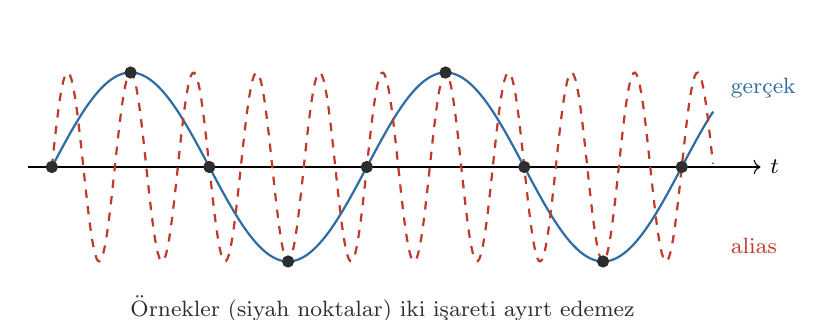
\begin{tikzpicture}[scale=1.0]
\draw[->] (-0.3,0)--(9.0,0) node[right]{\footnotesize $t$};
\draw[grafikMavi,thick,domain=0:8.4,samples=200] plot (\x,{1.2*sin(deg(2*pi*\x/4))});
\draw[kirmizi,thick,dashed,domain=0:8.4,samples=400] plot (\x,{1.2*sin(deg(2*pi*\x*1.25))});
\foreach \k in {0,1,...,8}{
  \pgfmathsetmacro{\xx}{\k}
  \filldraw[koyuGri] (\xx,{1.2*sin(deg(2*pi*\xx/4))}) circle (2pt);
}
\node[grafikMavi,right] at (8.5,1.0) {\footnotesize gerçek};
\node[kirmizi,right] at (8.5,-1.0) {\footnotesize alias};
\node[koyuGri] at (4.2,-1.8) {\footnotesize Örnekler (siyah noktalar) iki işareti ayırt edemez};
\end{tikzpicture}
\end{center}

\begin{lstlisting}
import numpy as np

fs = 1000.0                     # ornekleme frekansi
f1, f2 = 300.0, 700.0           # 700 = fs - 300  ->  ayni ornekler

n = np.arange(10)
x1 = np.sin(2*np.pi*f1*n/fs)
x2 = np.sin(2*np.pi*f2*n/fs)

print(np.max(np.abs(x1 + x2)))  # ~1e-15  ->  x2 = -x1  (isaret ters, ayni frekans)

# Genel alias kurali: gozlenen frekans
def alias_frekansi(f, fs):
    """f frekansinin fs ile orneklendiginde gorunecegi frekans (0..fs/2)."""
    f_mod = np.mod(f, fs)
    return np.where(f_mod > fs/2, fs - f_mod, f_mod)

for f in [100, 400, 600, 900, 1100, 1400]:
    print(f"{f:>5} Hz  ->  gorunen {alias_frekansi(f, 1000.0):>5.0f} Hz")
\end{lstlisting}

\begin{lstlisting}[style=outstyle]
  100 Hz  ->  gorunen   100 Hz
  400 Hz  ->  gorunen   400 Hz
  600 Hz  ->  gorunen   400 Hz
  900 Hz  ->  gorunen   100 Hz
 1100 Hz  ->  gorunen   100 Hz
 1400 Hz  ->  gorunen   400 Hz
\end{lstlisting}

\uyari{Aliasing \textbf{geri döndürülemez}. Örnekleme yapıldıktan sonra hangi
frekansın hangi aliası olduğunu ayırt etmenin yolu yoktur. Çözüm, ADC'den
\emph{önce} analog bir \textbf{anti-aliasing} alçak geçiren filtre koymaktır.
Aynı şey sayısal desimasyonda da geçerlidir: hız düşürmeden önce mutlaka
filtrele (Kısım 4).}

\gsub{Aliasing'i Duymak}

Aliasing'i en iyi kulakla anlarsın: frekansı sürekli artan bir chirp'i düşük
$f_s$ ile üretirsen, ses Nyquist'e ulaştığında ``geri döner''.

\begin{lstlisting}
import numpy as np, soundfile as sf

fs = 8000
t = np.arange(int(3*fs))/fs
# 0 Hz'den 8000 Hz'e giden chirp: Nyquist (4000) sonrasi geri katlanir
faz = 2*np.pi*np.cumsum(np.linspace(0, 8000, len(t)))/fs
x = 0.4*np.sin(faz)
sf.write('alias_chirp.wav', x.astype(np.float32), fs)

# Karsilastirma icin dogru yol: once yuksek fs'te uret, sonra filtreleyip indir
fs_hi = 48000
t_hi = np.arange(int(3*fs_hi))/fs_hi
faz_hi = 2*np.pi*np.cumsum(np.linspace(0, 8000, len(t_hi)))/fs_hi
x_hi = 0.4*np.sin(faz_hi)
from scipy import signal as sig
x_ok = sig.resample_poly(x_hi, up=1, down=6)      # anti-alias filtre dahil
sf.write('alias_yok.wav', x_ok.astype(np.float32), fs)
\end{lstlisting}

\ornek[Tekerlek Etkisi]{Filmlerde araba tekerleklerinin geriye dönüyormuş gibi
görünmesi tam olarak aliasing'dir: kamera saniyede 24 kare örnekler, teker
dönüş frekansı Nyquist'i (12 devir/s) aşınca alias frekansı negatif çıkar ve
teker geriye dönüyor görünür.}

% =====================================================================
\gsec{Kuantalama ve ADC}
% =====================================================================

Örnekleme zamanı kesikli yapar; \textbf{kuantalama} genliği kesikli yapar.
$b$ bitlik bir ADC, giriş aralığını $2^b$ seviyeye böler.

\form[Kuantalama Gürültüsü ve SQNR]{Adım büyüklüğü $\Delta=\dfrac{V_{pp}}{2^b}$
ise kuantalama hatası $[-\Delta/2,\Delta/2]$ aralığında düzgün dağılır ve
gücü $\sigma_q^2=\Delta^2/12$'dir. Tam ölçekli sinüs için
\[
\mathrm{SQNR}\ [\text{dB}] = 6{,}02\,b + 1{,}76 .
\]
Yani \textbf{her bit yaklaşık 6 dB} dinamik aralık kazandırır.}

\begin{lstlisting}
import numpy as np

def kuantala(x, bit, vmax=1.0):
    """x'i +-vmax araliginda bit-bitlik seviyelere yuvarlar (mid-tread)."""
    adim = 2*vmax/2**bit
    return np.clip(np.round(x/adim)*adim, -vmax, vmax - adim)

fs, f0 = 48000, 1000.0
t = np.arange(fs)/fs
x = 0.999*np.sin(2*np.pi*f0*t)

for b in [4, 8, 12, 16]:
    xq = kuantala(x, b)
    hata = xq - x
    sqnr = 10*np.log10(np.mean(x**2)/np.mean(hata**2))
    print(f"{b:>2} bit  SQNR = {sqnr:6.2f} dB   (teorik {6.02*b + 1.76:6.2f} dB)")
\end{lstlisting}

\begin{lstlisting}[style=outstyle]
 4 bit  SQNR =  24.40 dB   (teorik  25.84 dB)
 8 bit  SQNR =  49.59 dB   (teorik  49.92 dB)
12 bit  SQNR =  74.40 dB   (teorik  74.00 dB)
16 bit  SQNR =  97.24 dB   (teorik  98.08 dB)
\end{lstlisting}

\gsub{Dither: Gürültü Ekleyerek Kaliteyi Artırmak}

Çok düşük seviyeli işaretlerde kuantalama hatası işaretle \emph{ilişkilidir} ve
harmonik bozulma (çirkin, ``kırık'' bir ses) üretir. Kuantalamadan önce çok
küçük bir gürültü (\emph{dither}) eklemek bu hatayı ilişkisiz, düz bir gürültü
tabanına çevirir --- toplam gürültü artar ama bozulma duyulmaz olur.

\begin{lstlisting}
gurultu = np.random.uniform(-0.5, 0.5, len(x))*(2/2**8)    # 1 LSB genisliginde
x_dither = kuantala(x + gurultu, 8)
\end{lstlisting}

\bilgi{Aynı fikir \emph{gürültü şekillendirme} (noise shaping) ile birleşince
kuantalama gürültüsünü duyulmayan yüksek frekanslara itmeyi sağlar; CD
masteringinde ve $\Sigma\Delta$ (sigma-delta) ADC'lerde kullanılan yöntem
budur.}

% =====================================================================
\gsec{Karmaşık Sayılar ve Fazörler}
% =====================================================================

DSP'de karmaşık sayılar süs değil, zorunluluktur: bir sinüsün hem
\emph{genliğini} hem \emph{fazını} tek bir sayıda taşırlar ve negatif
frekansları temsil etmeyi mümkün kılarlar.

\form[Euler Formülü]{
\[
\ee^{\jj\theta}=\cos\theta+\jj\sin\theta,
\qquad
\cos\theta=\frac{\ee^{\jj\theta}+\ee^{-\jj\theta}}{2},
\qquad
\sin\theta=\frac{\ee^{\jj\theta}-\ee^{-\jj\theta}}{2\jj}.
\]
Bir \emph{fazör} $A\ee^{\jj(\omega n+\varphi)}$, karmaşık düzlemde sabit hızla
dönen bir vektördür: $A$ yarıçap, $\omega$ dönme hızı, $\varphi$ başlangıç
açısıdır.}

\begin{center}
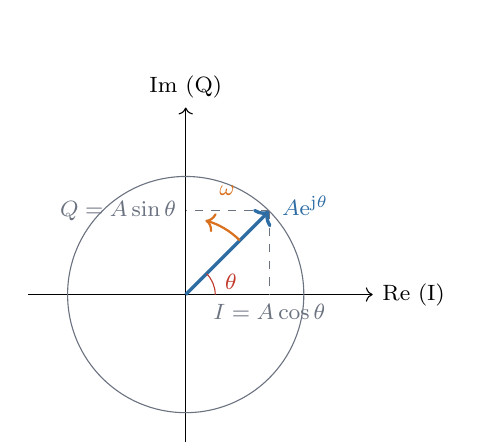
\begin{tikzpicture}[scale=1.25]
\draw[->] (-1.6,0)--(1.9,0) node[right]{\footnotesize Re (I)};
\draw[->] (0,-1.6)--(0,1.9) node[above]{\footnotesize Im (Q)};
\draw[ortaGri,thin] (0,0) circle (1.2);
\draw[grafikMavi,very thick,->] (0,0)--(0.85,0.85);
\draw[turuncu,thick,->] (0.55,0.55) arc (45:75:0.78);
\node[grafikMavi,right] at (0.88,0.9) {\footnotesize $A\ee^{\jj\theta}$};
\node[turuncu] at (0.42,1.05) {\footnotesize $\omega$};
\draw[dashed,ortaGri] (0.85,0.85)--(0.85,0) node[below]{\footnotesize $I=A\cos\theta$};
\draw[dashed,ortaGri] (0.85,0.85)--(0,0.85) node[left]{\footnotesize $Q=A\sin\theta$};
\draw[kirmizi] (0.3,0) arc (0:45:0.3);
\node[kirmizi,right] at (0.3,0.13) {\footnotesize $\theta$};
\end{tikzpicture}
\end{center}

\begin{lstlisting}
import numpy as np

z = 3 + 4j
print(abs(z), np.angle(z), np.angle(z, deg=True))   # 5.0  0.9273 rad  53.13 deg
print(z.real, z.imag, np.conj(z))                    # 3.0 4.0 (3-4j)

# Fazor uretme: en sik kullanacagin tek satir
fs, f0, N = 48000, 1000.0, 480
n = np.arange(N)
faz = np.exp(2j*np.pi*f0*n/fs)          # e^{j 2 pi f0 n / fs}

# Onemli ozellikler
print(np.allclose(np.abs(faz), 1.0))     # True  -> birim cemberde
print(np.allclose(faz.real, np.cos(2*np.pi*f0*n/fs)))   # True
\end{lstlisting}

\gsub{Neden Negatif Frekans Var?}

Gerçek bir kosinüs, zıt yönde dönen \emph{iki} fazörün toplamıdır:
\[
\cos(\omega n)=\tfrac12\ee^{\jj\omega n}+\tfrac12\ee^{-\jj\omega n}.
\]
Bu yüzden gerçek işaretlerin spektrumu her zaman simetriktir ($X[-f]=X^*[f]$)
ve bilginin yarısı gereksizdir. Karmaşık (IQ) işaretlerde ise pozitif ve
negatif frekanslar \emph{bağımsızdır}; bu da aynı örnekleme hızında iki kat
bant genişliği taşımayı sağlar. Kısım 4'ün tamamı bu fikrin üzerine kuruludur.

\begin{lstlisting}
N, fs = 1024, 1000.0
n = np.arange(N)

gercek   = np.cos(2*np.pi*100*n/fs)          # spektrumda +100 ve -100
karmasik = np.exp(2j*np.pi*100*n/fs)         # spektrumda yalnizca +100

for ad, x in [('gercek', gercek), ('karmasik', karmasik)]:
    X = np.fft.fftshift(np.abs(np.fft.fft(x)))
    f = np.fft.fftshift(np.fft.fftfreq(N, 1/fs))
    tepe = f[np.argsort(X)[-2:]]              # en buyuk iki tepe
    print(f"{ad:>9}: tepeler {np.sort(tepe)}")
# gercek: [-100.  100.]      karmasik: [ 99.6  100. ]  -> tek tepe
\end{lstlisting}

% =====================================================================
\gsec{Sinyal Üretimi ve WAV Dosyaları}
% =====================================================================

\gsub{Temel Dalga Biçimleri}

\begin{lstlisting}
import numpy as np
from scipy import signal as sig

fs = 48000
t = np.arange(int(1.0*fs))/fs

sinus     = np.sin(2*np.pi*440*t)
kare      = sig.square(2*np.pi*440*t, duty=0.5)
testere   = sig.sawtooth(2*np.pi*440*t)
ucgen     = sig.sawtooth(2*np.pi*440*t, width=0.5)
chirp     = sig.chirp(t, f0=100, f1=8000, t1=1.0, method='linear')
darbe     = sig.unit_impulse(len(t), 'mid')
beyaz     = np.random.default_rng(0).normal(0, 0.1, len(t))
\end{lstlisting}

\uyari{Kare ve testere dalgaları \emph{sonsuz} harmonik içerir; doğrudan
üretilirse Nyquist üstündeki harmonikler alias olur ve ses kirlenir. Temiz
sentez için ya bant-sınırlı üretim (BLIT/PolyBLEP) ya da yüksek hızda üretip
\code{resample\_poly} ile indirme kullanılır.}

\gsub{WAV Okuma ve Yazma}

\begin{lstlisting}
import soundfile as sf
import numpy as np

# Yazma: float32 [-1, 1] araliginda; kirpilmayi (clipping) onle
x = 0.5*np.sin(2*np.pi*440*np.arange(48000)/48000)
sf.write('la440.wav', x.astype(np.float32), 48000)

# Okuma: her zaman fs'i de al
y, fs = sf.read('la440.wav', dtype='float32')
print(y.shape, fs, y.dtype)          # (48000,) 48000 float32

# Stereo: (N, 2) sekilli dizi
stereo = np.stack([x, np.roll(x, 100)], axis=1)
sf.write('stereo.wav', stereo.astype(np.float32), 48000)
\end{lstlisting}

\begin{lstlisting}
# scipy alternatifi (ek bagimlilik istemiyorsan)
from scipy.io import wavfile

wavfile.write('int16.wav', 48000, (x*32767).astype(np.int16))
fs2, z = wavfile.read('int16.wav')
z = z.astype(np.float32)/32768.0     # normalize etmeyi UNUTMA
\end{lstlisting}

\ipucu{\code{scipy.io.wavfile} okuduğunda dosyadaki ham tipi (\code{int16})
verir; $\pm1$ aralığına \emph{sen} normalize etmelisin. \code{soundfile} ise
\code{dtype='float32'} ile bunu otomatik yapar --- bu yüzden rehber boyunca
\code{soundfile} tercih edilir.}

\gsub{Gerçek Zamanlı Ses Girişi/Çıkışı}

\begin{lstlisting}
import sounddevice as sd
import numpy as np

fs = 48000
# Cal
sd.play(0.3*np.sin(2*np.pi*440*np.arange(fs)/fs), fs); sd.wait()

# Kaydet (2 saniye, mono)
kayit = sd.rec(int(2*fs), samplerate=fs, channels=1, dtype='float32')
sd.wait()
kayit = kayit[:, 0]

# Akis (callback) ile gercek zamanli isleme
def callback(indata, outdata, frames, time, status):
    outdata[:] = 0.5*indata          # burada filtre/demodulasyon yapilir

with sd.Stream(samplerate=fs, blocksize=1024, channels=1, callback=callback):
    sd.sleep(5000)                   # 5 saniye calis
\end{lstlisting}

\uyari{Callback fonksiyonu \textbf{gerçek zamanlı} bir bağlamda çalışır:
içinde bellek ayırma, dosya G/Ç, \code{print} veya uzun hesap yapma. Aksi
hâlde ses kesilir (underrun). Ağır işi bir kuyruğa (\code{queue.Queue}) atıp
başka bir iş parçacığında yap.}

% #####################################################################
\gpart{2}{Frekans Alanı: DFT ve FFT}
% #####################################################################

% =====================================================================
\gsec{Fourier Fikri}
% =====================================================================

Fourier'in fikri tek cümleyle özetlenir: \textbf{her işaret, farklı
frekanslardaki sinüzoidlerin toplamı olarak yazılabilir.} Zaman alanında
karmaşık görünen bir problem (örneğin ``bu sesteki uğultuyu at'') frekans
alanında basitleşir (``50 Hz bileşenini sil'').

\form[Ayrık Fourier Dönüşümü (DFT)]{
\[
X[k]=\sum_{n=0}^{N-1}x[n]\,\ee^{-\jj 2\pi kn/N},
\qquad
x[n]=\frac{1}{N}\sum_{k=0}^{N-1}X[k]\,\ee^{\jj 2\pi kn/N}.
\]
$X[k]$, işaretin $f_k=k\,f_s/N$ frekansındaki bileşeninin genlik ve fazını
taşıyan karmaşık sayıdır.}

DFT'nin sezgisi bir \emph{iç çarpımdır}: işareti, her frekanstaki bir referans
fazörle çarpıp toplarız. İşarette o frekans varsa terimler birbirini
destekler ve büyük bir sayı çıkar; yoksa fazlar rastgele dağılır ve toplam
sıfıra yakın olur.

\gsub{DFT'yi Doğrudan Yazmak}

\begin{lstlisting}
import numpy as np

def dft_yavas(x):
    """Tanimdan DFT: O(N^2). Ogrenmek icin; uretimde asla kullanma."""
    x = np.asarray(x, dtype=complex)
    N = len(x)
    n = np.arange(N)
    k = n.reshape((N, 1))
    W = np.exp(-2j*np.pi*k*n/N)          # NxN donusum matrisi
    return W @ x

x = np.random.default_rng(0).normal(size=64)
print(np.allclose(dft_yavas(x), np.fft.fft(x)))     # True
\end{lstlisting}

\uyari{Matris yöntemi $N^2$ karmaşık sayı saklar: $N=10^5$ için 160 GB
bellek. Öğretici olarak güzeldir, pratikte kullanılamaz. Gerçek hayatta her
zaman \code{np.fft} (veya \code{scipy.fft}) kullan --- $O(N\log N)$.}

\gsub{Frekans Ekseni ve Ölçekleme}

En sık yapılan hata FFT çıktısını doğru frekansa ve doğru genliğe
eşleyememektir.

\begin{center}
\begin{tabularx}{\textwidth}{@{}>{\ttfamily\color{anaMavi}}l >{\raggedright\arraybackslash}X@{}}
\toprule
\rowcolor{acikMavi}\multicolumn{1}{@{}l}{\color{anaMavi}\textbf{Fonksiyon}} & \multicolumn{1}{l@{}}{\color{anaMavi}\textbf{Ne verir?}}\\
\midrule
np.fft.fft(x) & Karmaşık spektrum, $N$ nokta, $0\ldots f_s$ sırasıyla.\\
\rowcolor{acikGri} np.fft.rfft(x) & Gerçek girdi için yalnız pozitif frekanslar, $N/2+1$ nokta (2$\times$hızlı).\\
np.fft.fftfreq(N, 1/fs) & Frekans ekseni; ikinci yarısı negatif frekanslar.\\
\rowcolor{acikGri} np.fft.rfftfreq(N, 1/fs) & $0\ldots f_s/2$ arası frekans ekseni.\\
np.fft.fftshift(X) & Sıfır frekansı ortaya alır (IQ spektrumları için şart).\\
\rowcolor{acikGri} np.fft.ifft / irfft & Ters dönüşüm.\\
\bottomrule
\end{tabularx}
\end{center}

\form[Genlik Ölçekleme]{Genliği $A$ olan bir sinüs için FFT tepesi $NA/2$
büyüklüğündedir. Doğru genliği geri almak için:
\[
\text{tek yanlı genlik}=\frac{2\,|X[k]|}{N}
\qquad(k=0 \text{ ve } k=N/2 \text{ için } 2 \text{ çarpanı yok}).
\]
Pencere kullanılıyorsa $N$ yerine \emph{pencerenin toplamı} $\sum w[n]$ ile
böl.}

\begin{lstlisting}
import numpy as np

fs, N = 1000.0, 1000
n = np.arange(N)
x = 2.5*np.sin(2*np.pi*100*n/fs) + 1.0*np.sin(2*np.pi*250*n/fs)

X = np.fft.rfft(x)
f = np.fft.rfftfreq(N, 1/fs)
genlik = 2*np.abs(X)/N

for hedef in [100, 250]:
    k = np.argmin(np.abs(f - hedef))
    print(f"{f[k]:6.1f} Hz  ->  genlik {genlik[k]:.3f}")
\end{lstlisting}

\begin{lstlisting}[style=outstyle]
 100.0 Hz  ->  genlik 2.500
 250.0 Hz  ->  genlik 1.000
\end{lstlisting}

\gsub{Çözünürlük, Sızıntı ve Sıfır Doldurma}

\form[Frekans Çözünürlüğü]{
\[
\Delta f=\frac{f_s}{N}=\frac{1}{T}
\]
Burada $T=N/f_s$ \emph{gözlem süresidir}. Çözünürlüğü artırmanın tek yolu
daha uzun süre gözlemektir; sıfır doldurma (zero-padding) çözünürlük
\emph{kazandırmaz}, sadece spektrumu daha sık örnekler (interpolasyon).}

\begin{lstlisting}
fs = 1000.0
for N in [100, 1000, 10000]:
    print(f"N={N:>6}  T={N/fs:6.2f} s  df={fs/N:6.2f} Hz")
# N=   100  T=  0.10 s  df= 10.00 Hz
# N=  1000  T=  1.00 s  df=  1.00 Hz
# N= 10000  T= 10.00 s  df=  0.10 Hz

# Sifir doldurma: tepe konumunu daha iyi okumak icin
x = np.sin(2*np.pi*100.5*np.arange(256)/fs)
X1 = np.abs(np.fft.rfft(x))                 # 129 nokta
X2 = np.abs(np.fft.rfft(x, n=4096))         # 2049 nokta, ayni bilgi
\end{lstlisting}

\uyari{FFT, işaretin \emph{periyodik} olduğunu varsayar. Pencere sınırında
işaret kendine düzgün eklenmiyorsa (frekans, bin merkezine denk gelmiyorsa)
kesme süreksizliği spektrumda \textbf{sızıntı} (spectral leakage) üretir:
tek bir sinüs, tüm spektruma yayılır. Çözüm pencerelemedir.}

% =====================================================================
\gsec{FFT: Hızlı Fourier Dönüşümü}
% =====================================================================

FFT bir dönüşüm değil, DFT'yi hesaplamanın hızlı bir \emph{algoritmasıdır}.
Temel fikir böl-ve-fethet: $N$ noktalı DFT, çift ve tek indisli örneklerin
$N/2$ noktalı iki DFT'sine indirgenir.

\form[Radix-2 Kelebek (Butterfly)]{
\[
X[k]=E[k]+\ee^{-\jj2\pi k/N}O[k],
\qquad
X[k+N/2]=E[k]-\ee^{-\jj2\pi k/N}O[k]
\]
$E$: çift indisli örneklerin DFT'si, $O$: tek indislilerin. Karmaşıklık
$O(N^2)\to O(N\log N)$'e iner.}

\begin{lstlisting}
import numpy as np

def fft_radix2(x):
    """Ozyinelemeli radix-2 FFT. N ikinin kuvveti olmali."""
    x = np.asarray(x, dtype=complex)
    N = len(x)
    if N & (N - 1):
        raise ValueError("N ikinin kuvveti olmali")
    if N == 1:
        return x
    cift = fft_radix2(x[0::2])
    tek  = fft_radix2(x[1::2])
    W = np.exp(-2j*np.pi*np.arange(N//2)/N)      # twiddle carpanlari
    return np.concatenate([cift + W*tek, cift - W*tek])

x = np.random.default_rng(1).normal(size=1024)
print(np.allclose(fft_radix2(x), np.fft.fft(x)))    # True
\end{lstlisting}

\gsub{Yerinde (In-Place) Yinelemeli FFT}

Özyinelemeli sürüm her adımda yeni dizi ayırır. Üretim uygulamaları
\emph{yerinde} çalışır: önce girdiyi bit-ters (bit-reversal) sıraya dizer,
sonra $\log_2 N$ kademede kelebekleri uygular.

\begin{lstlisting}
import numpy as np

def bit_ters_permutasyon(N):
    """0..N-1 icin bit-ters indeks tablosu (N ikinin kuvveti)."""
    bit = int(np.log2(N))
    idx = np.arange(N)
    ters = np.zeros(N, dtype=int)
    for b in range(bit):
        ters |= ((idx >> b) & 1) << (bit - 1 - b)
    return ters

def fft_yerinde(x):
    """Yinelemeli radix-2 FFT: kademe kademe, ek dizi ayirmadan."""
    x = np.asarray(x, dtype=complex).copy()
    N = len(x)
    if N & (N - 1):
        raise ValueError("N ikinin kuvveti olmali")

    x = x[bit_ters_permutasyon(N)]              # 1) bit-ters siralama

    adim = 2
    while adim <= N:                             # 2) log2(N) kademe
        W = np.exp(-2j*np.pi*np.arange(adim//2)/adim)
        for bas in range(0, N, adim):
            ust = x[bas:bas + adim//2].copy()
            alt = x[bas + adim//2:bas + adim]*W
            x[bas:bas + adim//2] = ust + alt      # kelebek
            x[bas + adim//2:bas + adim] = ust - alt
        adim *= 2
    return x

x = np.random.default_rng(3).normal(size=2048)
print(np.allclose(fft_yerinde(x), np.fft.fft(x)))     # True
\end{lstlisting}

\bilgi{Bit-ters sıralamanın nedeni, böl-ve-fethetin çift/tek ayrımını tersten
uygulamaktır: özyinelemede ``önce böl, sonra birleştir'' yapılan iş,
yinelemeli sürümde ``önce doğru sıraya diz, sonra birleştir'' hâline gelir.
Bu, FFTW ve pocketfft gibi kütüphanelerin de temel yapısıdır --- üstüne SIMD,
önbellek blokları ve karışık radix eklenmiştir.}

\gsub{Hız Karşılaştırması}

\begin{lstlisting}
import numpy as np, time

x = np.random.default_rng(0).normal(size=4096)

def sure_olc(fn, tekrar=20):
    t0 = time.perf_counter()
    for _ in range(tekrar):
        fn(x)
    return (time.perf_counter() - t0)/tekrar*1e3     # ms

print(f"dft_yavas   : {sure_olc(dft_yavas, 3):8.2f} ms")
print(f"fft_radix2  : {sure_olc(fft_radix2):8.2f} ms")
print(f"np.fft.fft  : {sure_olc(np.fft.fft):8.2f} ms")
print(f"np.fft.rfft : {sure_olc(np.fft.rfft):8.2f} ms")
\end{lstlisting}

\begin{lstlisting}[style=outstyle]
dft_yavas   :   210.44 ms
fft_radix2  :    12.83 ms
np.fft.fft  :     0.06 ms
np.fft.rfft :     0.03 ms
\end{lstlisting}

\ipucu{Kütüphane FFT'si kendi yazdığından yüzlerce kat hızlıdır: SIMD, önbellek
dostu erişim ve karışık radix (2,3,5,7) desteği vardır. \code{scipy.fft} ayrıca
\code{workers=-1} ile çok çekirdek kullanır. Uzunluğu \code{next\_fast\_len}
ile yuvarlamak, asal uzunluklu FFT'lerdeki yavaşlığı önler.}

\begin{lstlisting}
from scipy import fft as spfft

N = 10007                                 # asal uzunluk: yavas
Nf = spfft.next_fast_len(N)               # 10080 gibi 2/3/5-carpanli sayi
X = spfft.fft(x, n=Nf, workers=-1)        # cok cekirdekli
\end{lstlisting}

% =====================================================================
\gsec{Pencereleme (Windowing)}
% =====================================================================

Pencereleme, kesme süreksizliğini yumuşatarak sızıntıyı azaltır. Bedeli, ana
lobun genişlemesi --- yani \emph{çözünürlük} ile \emph{dinamik aralık}
arasında bir takas yaparız.

\begin{center}
\begin{tabularx}{\textwidth}{@{}>{\ttfamily\color{anaMavi}}l c c >{\raggedright\arraybackslash}X@{}}
\toprule
\rowcolor{acikMavi}\multicolumn{1}{@{}l}{\color{anaMavi}\textbf{Pencere}} & \multicolumn{1}{c}{\color{anaMavi}\textbf{Yan lob}} & \multicolumn{1}{c}{\color{anaMavi}\textbf{Ana lob}} & \multicolumn{1}{l@{}}{\color{anaMavi}\textbf{Ne zaman?}}\\
\midrule
boxcar & $-13$ dB & 1,0 bin & En iyi çözünürlük, en kötü sızıntı.\\
\rowcolor{acikGri} hann & $-31$ dB & 2,0 bin & Genel amaçlı varsayılan.\\
hamming & $-43$ dB & 2,0 bin & İlk yan lobu bastırır.\\
\rowcolor{acikGri} blackman & $-58$ dB & 3,0 bin & Yüksek dinamik aralık.\\
blackmanharris & $-92$ dB & 4,0 bin & Çok zayıf işaretleri görmek için.\\
\rowcolor{acikGri} kaiser($\beta$) & ayarlanır & ayarlanır & $\beta$ ile takası sen seç.\\
flattop & $-88$ dB & 4,7 bin & Genlik ölçümü (tepe hatası $<0{,}01$ dB).\\
\bottomrule
\end{tabularx}
\end{center}

\begin{lstlisting}
import numpy as np
from scipy import signal as sig

fs, N = 1000.0, 1024
n = np.arange(N)
# Bin merkezine denk GELMEYEN bir frekans: sizinti gorunur
x = np.sin(2*np.pi*100.5*n/fs) + 1e-4*np.sin(2*np.pi*250*n/fs)    # -80 dB komsu

for ad in ['boxcar', 'hann', 'blackmanharris']:
    w = sig.get_window(ad, N)
    X = np.fft.rfft(x*w)
    mag = 20*np.log10(np.abs(X)/np.sum(w)*2 + 1e-15)
    f = np.fft.rfftfreq(N, 1/fs)
    k = np.argmin(np.abs(f - 250))
    print(f"{ad:>15}: 250 Hz'te okunan seviye = {mag[k]:7.2f} dB")
\end{lstlisting}

\begin{lstlisting}[style=outstyle]
         boxcar: 250 Hz'te okunan seviye =  -61.51 dB
           hann: 250 Hz'te okunan seviye =  -80.00 dB
 blackmanharris: 250 Hz'te okunan seviye =  -79.99 dB
\end{lstlisting}

Dikdörtgen pencerede $-80$ dB'lik zayıf işaret, güçlü komşunun sızıntısı
altında kalıyor ve $18$ dB yanlış (çok güçlü) okunuyor. Hann ve
Blackman-Harris ile seviye doğru çıkıyor --- pencereleme burada bir süsleme
değil, ölçümün doğru olup olmamasının farkı.

\form[Pencere Kazançları]{İki farklı normalizasyon vardır ve karıştırılırsa
sonuç birkaç dB kayar:
\[
\text{tutarlı kazanç (genlik için)}=\frac{1}{N}\sum_n w[n],
\qquad
\text{güç kazancı (PSD için)}=\frac{1}{N}\sum_n w^2[n].
\]}

% =====================================================================
\gsec{Güç Spektral Yoğunluğu ve Spektrogram}
% =====================================================================

Tek bir FFT gürültülü bir kestirimdir: varyansı, veri uzunluğundan bağımsız
olarak ortalamanın kendisi kadardır. \textbf{Welch yöntemi}, işareti örtüşen
bloklara böler, her birinin periyodogramını alır ve ortalar --- gürültü
tabanı düzleşir.

\begin{lstlisting}
import numpy as np
from scipy import signal as sig
import matplotlib.pyplot as plt

fs = 48000
t = np.arange(4*fs)/fs
x = (np.sin(2*np.pi*1000*t) + 0.01*np.sin(2*np.pi*3000*t)
     + np.random.default_rng(0).normal(0, 0.05, len(t)))

# Periyodogram (tek FFT) vs Welch (ortalamali)
f1, P1 = sig.periodogram(x, fs, window='hann', scaling='density')
f2, P2 = sig.welch(x, fs, nperseg=4096, noverlap=2048, scaling='density')

plt.semilogy(f1, P1, lw=0.5, alpha=0.5, label='periyodogram')
plt.semilogy(f2, P2, lw=1.5, label='Welch')
plt.xlim(0, 6000); plt.legend(); plt.grid(alpha=0.3)
plt.xlabel('Hz'); plt.ylabel('PSD (V^2/Hz)'); plt.show()
\end{lstlisting}

\bilgi{\code{scaling='density'} sonucu V$^2$/Hz olarak verir (gürültü tabanı
karşılaştırmaları için); \code{scaling='spectrum'} ise V$^2$ verir (ayrık
tonların gücünü okumak için). Toplam gücü doğrulamak istersen Parseval'i
kullan: \code{np.trapz(P, f)} $\approx$ \code{np.mean(x**2)}.}

\gsub{Spektrogram: Zaman-Frekans Görüntüsü}

\begin{lstlisting}
f, tt, Sxx = sig.spectrogram(x, fs, window='hann', nperseg=1024,
                             noverlap=768, scaling='density', mode='psd')
plt.pcolormesh(tt, f, 10*np.log10(Sxx + 1e-15), shading='gouraud',
               cmap='magma', vmin=-120, vmax=-20)
plt.ylabel('Frekans (Hz)'); plt.xlabel('Zaman (s)')
plt.colorbar(label='dB'); plt.ylim(0, 6000); plt.show()
\end{lstlisting}

\form[Zaman--Frekans Takası]{Blok uzunluğu $M$ için
\[
\Delta f=\frac{f_s}{M},\qquad \Delta t=\frac{M}{f_s}
\quad\Longrightarrow\quad \Delta f\cdot\Delta t=1 .
\]
Frekansta netlik istiyorsan zamanda bulanıklaşırsın; bu, DSP'nin
belirsizlik ilkesidir. Konuşma için $\sim$25 ms, radyo sinyalleri için
$\sim$1--10 ms tipik seçimlerdir.}

\gsub{IQ İşaretlerin Spektrumu}

Karmaşık işaretlerde spektrum simetrik \emph{değildir}; negatif frekanslar
gerçek bilgi taşır. Bu yüzden \code{fftshift} ve \code{return\_onesided=False}
şarttır.

\begin{lstlisting}
fs = 2.4e6                                   # SDR ornekleme hizi
iq = ...                                     # complex64 dizi

f, P = sig.welch(iq, fs, nperseg=4096, return_onesided=False, scaling='density')
f = np.fft.fftshift(f); P = np.fft.fftshift(P)
plt.plot(f/1e6, 10*np.log10(P + 1e-20))
plt.xlabel('Ara frekans (MHz)'); plt.ylabel('dB'); plt.grid(alpha=0.3); plt.show()
\end{lstlisting}

\uyari{Gerçek işaret için \code{rfft}, karmaşık işaret için \code{fft} +
\code{fftshift} kullan. Karmaşık bir IQ akışına \code{rfft} uygularsan
negatif frekans bilgisini sessizce kaybedersin --- spektrum ``doğru
görünür'' ama yanlıştır.}

% #####################################################################
\gpart{3}{Filtreler: FIR ve IIR}
% #####################################################################

% =====================================================================
\gsec{Konvolüsyon ve FIR Filtreler}
% =====================================================================

Doğrusal ve zamanla değişmeyen (LTI) her sistem \textbf{konvolüsyonla}
tanımlanır. Sistemin dürtü yanıtı $h[n]$ ise çıkış:
\[
y[n]=\sum_{k}h[k]\,x[n-k]=(h*x)[n].
\]

\form[Konvolüsyon Teoremi]{Zaman alanındaki konvolüsyon, frekans alanında
\emph{çarpmadır}:
\[
y=h*x \quad\Longleftrightarrow\quad Y(f)=H(f)\,X(f).
\]
Bu yüzden filtreleme, spektrumu $H(f)$ ile şekillendirmek demektir.}

\gsub{NumPy/SciPy ile Konvolüsyon}

\begin{center}
\begin{tabularx}{\textwidth}{@{}>{\ttfamily\color{anaMavi}}l >{\raggedright\arraybackslash}X@{}}
\toprule
\rowcolor{acikMavi}\multicolumn{1}{@{}l}{\color{anaMavi}\textbf{Fonksiyon}} & \multicolumn{1}{l@{}}{\color{anaMavi}\textbf{Ne zaman?}}\\
\midrule
np.convolve(x,h) & Kısa filtreler ($<$100 katsayı), tek seferlik işler.\\
\rowcolor{acikGri} sig.convolve(x,h,method='auto') & Uzunluğa bakıp doğrudan/FFT yöntemini kendi seçer.\\
sig.fftconvolve(x,h) & Uzun filtreler; $O(N\log N)$.\\
\rowcolor{acikGri} sig.lfilter(b,a,x) & Nedensel, durum taşıyabilen (blok blok) filtreleme.\\
sig.oaconvolve(x,h) & Çok uzun akışlar için overlap-add.\\
\rowcolor{acikGri} sig.filtfilt(b,a,x) & İleri-geri: \textbf{sıfır faz}, gecikme yok (çevrimdışı).\\
\bottomrule
\end{tabularx}
\end{center}

\begin{lstlisting}
import numpy as np
from scipy import signal as sig

x = np.random.default_rng(0).normal(size=100_000)
h = sig.firwin(301, 0.2)

y1 = np.convolve(x, h, mode='same')          # yavas ama basit
y2 = sig.fftconvolve(x, h, mode='same')      # cok daha hizli
y3 = sig.lfilter(h, 1.0, x)                  # nedensel, (len(h)-1)/2 gecikmeli

print(np.allclose(y1, y2))                   # True
\end{lstlisting}

\uyari{\code{mode} parametresi çıkış uzunluğunu belirler: \code{'full'}
($N+M-1$), \code{'same'} ($N$, ortadan hizalı), \code{'valid'} ($N-M+1$,
yalnız tam örtüşen kısım). Hizalama hatası, ölçümlerinde yarım filtre
uzunluğu kadar gecikme olarak karşına çıkar.}

\gsub{FIR Filtrenin Doğrusal Fazı}

FIR katsayıları simetrikse ($h[n]=h[M-1-n]$) filtre \textbf{doğrusal fazlıdır}:
bütün frekanslar aynı miktarda gecikir, dalga biçimi bozulmaz. Gecikme tam
olarak $(M-1)/2$ örnektir.

\begin{center}
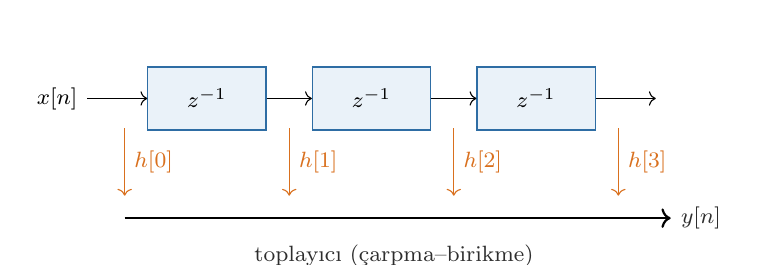
\begin{tikzpicture}[scale=0.95, every node/.style={font=\footnotesize}]
\node[draw=vurguMavi,fill=acikMavi,minimum width=1.5cm,minimum height=0.8cm] (z1) at (0,0) {$z^{-1}$};
\node[draw=vurguMavi,fill=acikMavi,minimum width=1.5cm,minimum height=0.8cm] (z2) at (2.2,0) {$z^{-1}$};
\node[draw=vurguMavi,fill=acikMavi,minimum width=1.5cm,minimum height=0.8cm] (z3) at (4.4,0) {$z^{-1}$};
\draw[->] (-1.6,0)--(z1); \draw[->] (z1)--(z2); \draw[->] (z2)--(z3); \draw[->] (z3)--(6.0,0);
\node[left] at (-1.6,0) {$x[n]$};
\foreach \i/\p in {0/-1.1, 1/1.1, 2/3.3, 3/5.5}{
  \draw[->,turuncu] (\p,-0.4)--(\p,-1.3);
  \node[turuncu,right] at (\p,-0.85) {$h[\i]$};
}
\draw[->,thick] (-1.1,-1.6)--(6.2,-1.6) node[right,koyuGri] {$y[n]$};
\node[koyuGri] at (2.5,-2.1) {toplayıcı (çarpma--birikme)};
\end{tikzpicture}
\end{center}

\gsub{Pencere Yöntemiyle Alçak Geçiren Tasarım}

İdeal alçak geçiren filtrenin dürtü yanıtı bir \emph{sinc}'tir; sonsuz uzun
olduğu için kesip pencereleriz.

\form[Kesilmiş Sinc]{
\[
h[n]=2f_c\,\mathrm{sinc}\!\big(2f_c(n-M/2)\big)\cdot w[n],
\qquad f_c=\frac{f_{\text{kesim}}}{f_s}
\]}

\begin{lstlisting}
import numpy as np
from scipy import signal as sig

def alcak_gecen_fir(kesim_hz, fs, taps=101, pencere='hamming'):
    """Pencere yontemiyle alcak gecirgen FIR (elle, ogretici)."""
    fc = kesim_hz/fs                              # normalize kesim (0..0.5)
    n = np.arange(taps) - (taps - 1)/2
    h = 2*fc*np.sinc(2*fc*n)                      # np.sinc(x) = sin(pi x)/(pi x)
    h *= sig.get_window(pencere, taps)
    return h/np.sum(h)                             # DC kazanci 1 olsun

h_elle = alcak_gecen_fir(1000, 48000, 101)
h_scipy = sig.firwin(101, 1000, fs=48000, window='hamming')
print(np.allclose(h_elle, h_scipy))                # True
\end{lstlisting}

\gsub{Filtreyi Doğrulamak: Frekans Yanıtı}

\begin{lstlisting}
import matplotlib.pyplot as plt

w, H = sig.freqz(h_scipy, worN=8192, fs=48000)

fig, (a1, a2) = plt.subplots(2, 1, figsize=(7, 6), sharex=True)
a1.plot(w, 20*np.log10(np.abs(H) + 1e-12), color='#2E6DA4')
a1.set_ylabel('Genlik (dB)'); a1.set_ylim(-100, 5); a1.grid(alpha=0.3)
a1.axvline(1000, ls='--', color='#C0392B')
a2.plot(w, np.unwrap(np.angle(H)), color='#D9701E')
a2.set_ylabel('Faz (rad)'); a2.set_xlabel('Hz'); a2.grid(alpha=0.3)
plt.show()

# Grup gecikmesi: dogrusal fazli FIR'de sabit olmali
wg, gd = sig.group_delay((h_scipy, 1.0), fs=48000)
print(np.round(gd[:5], 3))     # [50. 50. 50. 50. 50.]  -> (101-1)/2
\end{lstlisting}

\gsub{Tasarım Parametreleri: Kaç Katsayı Gerekir?}

\form[Kaiser Tahmini]{Geçiş bandı genişliği $\Delta f$ ve durdurma bandı
bastırması $A$ dB için gereken katsayı sayısı yaklaşık
\[
M\approx\frac{A-8}{2{,}285\cdot 2\pi\,\Delta f/f_s}.
\]
Yani \textbf{keskin geçiş pahalıdır}: geçiş bandını yarıya indirmek katsayı
sayısını iki katına çıkarır.}

\begin{lstlisting}
from scipy.signal import kaiserord, firwin, remez

fs = 48000
gecis = 500.0          # gecis bandi genisligi (Hz)
A = 60.0               # istenen bastirma (dB)

M, beta = kaiserord(A, gecis/(fs/2))
print(f"gereken katsayi: {M}, kaiser beta = {beta:.3f}")
h = firwin(M, 1000, window=('kaiser', beta), fs=fs)

# Alternatif: Parks-McClellan (esdalgali, ayni bastirma icin en az katsayi)
h_pm = remez(M, [0, 1000, 1500, fs/2], [1, 0], fs=fs)
\end{lstlisting}

\ipucu{\code{remez} (Parks--McClellan) aynı şartname için pencere yönteminden
\%20--30 daha az katsayı kullanır; hesap yükünün kritik olduğu gerçek zamanlı
hatlarda tercih edilir. Ama yakınsamayabilir --- tasarımı her zaman
\code{freqz} ile doğrula.}

% =====================================================================
\gsec{IIR Filtreler, SOS ve Sıfır Faz}
% =====================================================================

IIR filtreler geri besleme kullanır: çok daha az katsayıyla keskin geçiş
verirler, ama fazları doğrusal değildir ve kararsız olabilirler.

\form[IIR Fark Denklemi]{
\[
y[n]=\sum_{k=0}^{P}b_k x[n-k]-\sum_{k=1}^{Q}a_k y[n-k],
\qquad
H(z)=\frac{b_0+b_1z^{-1}+\dots}{1+a_1z^{-1}+\dots}
\]}

\begin{center}
\begin{tabularx}{\textwidth}{@{}>{\bfseries\color{anaMavi}}l >{\raggedright\arraybackslash}X@{}}
\toprule
\rowcolor{acikMavi}\multicolumn{1}{@{}l}{\color{anaMavi}\textbf{Tip}} & \multicolumn{1}{l@{}}{\color{anaMavi}\textbf{Karakteri}}\\
\midrule
Butterworth & Geçiş bandı maksimum düz; en yumuşak geçiş.\\
\rowcolor{acikGri} Chebyshev I & Geçiş bandında dalgalanma, daha keskin geçiş.\\
Chebyshev II & Durdurma bandında dalgalanma, geçiş bandı düz.\\
\rowcolor{acikGri} Elliptic (Cauer) & İki bantta da dalgalanma; verilen derece için en keskin.\\
Bessel & Neredeyse doğrusal faz; dalga biçimini korur (darbeler için).\\
\bottomrule
\end{tabularx}
\end{center}

\begin{lstlisting}
import numpy as np
from scipy import signal as sig

fs = 48000
# HER ZAMAN sos (second-order sections) formati kullan: sayisal olarak kararli
sos = sig.butter(8, 1000, btype='low', fs=fs, output='sos')
y = sig.sosfilt(sos, x)                    # nedensel (gercek zamanli)
y0 = sig.sosfiltfilt(sos, x)               # ileri-geri: sifir faz, 2x dik

# Bant geciren / bant durduran
sos_bp = sig.butter(6, [300, 3400], btype='bandpass', fs=fs, output='sos')
b_no, a_no = sig.iirnotch(50.0, Q=30, fs=fs)         # sebeke ugultusu (b, a)

# Kararlilik ve kutup-sifir kontrolu
z, p, k = sig.sos2zpk(sos)
print('en buyuk kutup yaricapi:', np.max(np.abs(p)))  # < 1 olmali
\end{lstlisting}

\uyari{\code{output='ba'} (tek payda polinomu) yüksek dereceli filtrelerde
\textbf{sayısal olarak patlar}: 8. dereceden sonra katsayılar arasındaki
büyüklük farkı çift duyarlığı aşar ve filtre kararsızlaşır. Her zaman
\code{output='sos'} kullan ve \code{sosfilt}/\code{sosfiltfilt} ile uygula.}

\gsub{Sıfır Faz: filtfilt}

\code{filtfilt} işareti önce ileri, sonra geri filtreler. Sonuç: faz
bozulması tam olarak sıfır, genlik yanıtı ise karesi alınmış hâli (bastırma
iki katı). Bedeli, nedensel olmamasıdır --- yalnızca kayıtlı veride kullanılır.

\begin{lstlisting}
y_ileri = sig.sosfilt(sos, x)        # gecikmeli (grup gecikmesi kadar)
y_sifir = sig.sosfiltfilt(sos, x)    # gecikmesiz, gercek zamanda KULLANILAMAZ
\end{lstlisting}

\gsub{Biquad: IIR'ın Yapı Taşı}

\begin{lstlisting}
def biquad_lowpass(f0, fs, Q=0.7071):
    """Audio EQ Cookbook alcak gecirgen biquad katsayilari."""
    w0 = 2*np.pi*f0/fs
    alpha = np.sin(w0)/(2*Q)
    cw = np.cos(w0)
    b = np.array([(1 - cw)/2, 1 - cw, (1 - cw)/2])
    a = np.array([1 + alpha, -2*cw, 1 - alpha])
    return b/a[0], a/a[0]

b, a = biquad_lowpass(1000, 48000)
w, H = sig.freqz(b, a, worN=4096, fs=48000)
\end{lstlisting}

% =====================================================================
\gsec{Ucuz Filtreler: Hareketli Ortalama, CIC, DC Engelleyici}
% =====================================================================

\gsub{Hareketli Ortalama}

En basit alçak geçiren filtre: son $M$ örneğin ortalaması. Kümülatif toplamla
$O(1)$ maliyetle uygulanır.

\begin{lstlisting}
def hareketli_ortalama(x, M):
    """cumsum hilesiyle O(N) hareketli ortalama."""
    c = np.cumsum(np.insert(x, 0, 0.0))
    return (c[M:] - c[:-M])/M

# Frekans yaniti: sinc bicimli, ilk sifir fs/M'de
M = 16
w, H = sig.freqz(np.ones(M)/M, 1.0, worN=4096, fs=48000)
\end{lstlisting}

\uyari{Hareketli ortalamanın durdurma bandı bastırması yalnızca $-13$ dB'dir;
yan lobları çok yüksektir. Ucuzdur ama ``iyi filtre'' değildir --- seçicilik
gerekiyorsa FIR/IIR kullan. Ard arda 3--5 kez uygulamak (kaskad) yan lobları
belirgin biçimde bastırır.}

\gsub{CIC (Cascaded Integrator-Comb)}

Çarpma içermeyen, yalnızca toplama-çıkarma kullanan desimasyon filtresi;
FPGA ve SDR ön uçlarının vazgeçilmezi.

\begin{lstlisting}
def cic_desimasyon(x, R, N=3):
    """R kat desimasyon, N mertebeli CIC (carpma yok)."""
    y = x.astype(np.float64)
    for _ in range(N):                     # integratorler
        y = np.cumsum(y)
    y = y[::R]                              # hiz dusurme
    for _ in range(N):                      # comb (fark) asamalari
        y = np.diff(y, prepend=0.0)
    return y/(R**N)                         # kazanc telafisi
\end{lstlisting}

\gsub{DC Engelleyici}

Ortalamayı (0 Hz bileşenini) süzen tek kutuplu yüksek geçiren:
\[
y[n]=x[n]-x[n-1]+\alpha\,y[n-1],\qquad \alpha\approx0{,}995 .
\]

\begin{lstlisting}
def dc_engelle(x, alpha=0.995):
    return sig.lfilter([1, -1], [1, -alpha], x)
\end{lstlisting}

\bilgi{RTL-SDR gibi doğrudan dönüştürücü alıcılarda merkez frekansta güçlü bir
\textbf{DC tepesi} bulunur (LO sızıntısı). Bu tepe demodülasyonu bozar; ya
DC engelleyiciyle süzülür ya da ilgilenilen kanal biraz kaydırılarak (offset
tuning) DC'den uzaklaştırılır.}

% =====================================================================
\gsec{Akış İşleme: Blok Blok Filtreleme}
% =====================================================================

Gerçek zamanlı sistemlerde veri parça parça gelir. Filtre durumunu bloklar
arasında taşımazsan her blok sınırında tıklama sesi duyarsın.

\begin{lstlisting}
import numpy as np
from scipy import signal as sig

sos = sig.butter(6, 3000, fs=48000, output='sos')
zi = sig.sosfilt_zi(sos)*0.0          # baslangic durumu (sifir)

def blok_isle(blok):
    global zi
    y, zi = sig.sosfilt(sos, blok, zi=zi)      # durum tasinir
    return y

# 1024'luk bloklarla akis
akis = np.random.default_rng(0).normal(size=48000)
cikis = np.concatenate([blok_isle(akis[i:i+1024])
                        for i in range(0, len(akis), 1024)])

# Dogrulama: tek seferde filtrelemekle ayni sonuc
print(np.allclose(cikis, sig.sosfilt(sos, akis)))     # True
\end{lstlisting}

\ipucu{FIR için aynı iş \code{sig.lfilter(h, 1.0, blok, zi=zi)} ile yapılır;
uzun FIR'lerde \code{sig.oaconvolve} (overlap-add) daha hızlıdır. Overlap-add
mantığı: her bloğu FFT ile filtrele, taşan $M-1$ örneği bir sonraki bloğa
ekle.}

\begin{lstlisting}
def overlap_add(x, h, blok=4096):
    """Elle overlap-add: uzun FIR'i FFT ile blok blok uygular."""
    M = len(h)
    Nf = 1 << int(np.ceil(np.log2(blok + M - 1)))
    H = np.fft.rfft(h, Nf)
    y = np.zeros(len(x) + M - 1)
    for i in range(0, len(x), blok):
        parca = x[i:i+blok]
        Y = np.fft.irfft(np.fft.rfft(parca, Nf)*H, Nf)
        y[i:i+len(Y)] += Y[:len(y) - i]
    return y[:len(x)]
\end{lstlisting}

% #####################################################################
\gpart{4}{IQ ve Karmaşık Bant Temeli}
% #####################################################################

% =====================================================================
\gsec{IQ Nedir? Analitik İşaret}
% =====================================================================

Modern telsiz haberleşmenin tamamı tek bir fikre dayanır: yüksek frekanslı
gerçek bir işareti, \emph{karmaşık} ve düşük hızlı bir işarete indirgemek.
Bu karmaşık işarete \textbf{bant temeli} (baseband) ya da \textbf{IQ} denir.

\form[IQ Gösterimi]{
\[
s(t)=A(t)\cos\!\big(2\pi f_c t+\varphi(t)\big)
= \Re\Big\{\underbrace{A(t)\ee^{\jj\varphi(t)}}_{\text{bant temeli } z(t)}
\;\ee^{\jj2\pi f_ct}\Big\}
\]
\[
z(t)=I(t)+\jj Q(t),\qquad
I=A\cos\varphi,\quad Q=A\sin\varphi,\quad
A=|z|,\quad \varphi=\arg z .
\]
Yani $I$ ve $Q$, taşıyıcının genlik ve fazını taşıyan iki gerçek kanaldır.}

\begin{center}
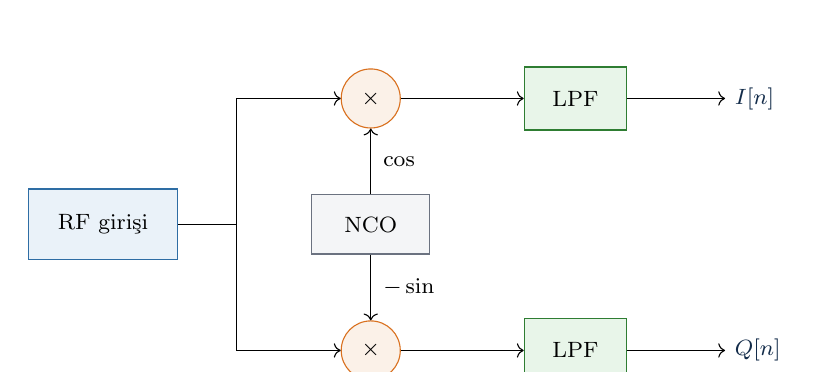
\begin{tikzpicture}[scale=1.0, every node/.style={font=\footnotesize}]
\node[draw=vurguMavi,fill=acikMavi,minimum width=1.9cm,minimum height=0.9cm] (rf) at (0,0) {RF girişi};
\node[draw=turuncu,fill=turuncu!10,circle,minimum size=0.75cm] (m1) at (3.4,1.6) {$\times$};
\node[draw=turuncu,fill=turuncu!10,circle,minimum size=0.75cm] (m2) at (3.4,-1.6) {$\times$};
\node[draw=yesil,fill=acikYesil,minimum width=1.3cm,minimum height=0.8cm] (l1) at (6.0,1.6) {LPF};
\node[draw=yesil,fill=acikYesil,minimum width=1.3cm,minimum height=0.8cm] (l2) at (6.0,-1.6) {LPF};
\node[draw=ortaGri,fill=acikGri,minimum width=1.5cm,minimum height=0.75cm] (osc) at (3.4,0) {NCO};
\draw[->] (rf)--(1.7,0)--(1.7,1.6)--(m1);
\draw[->] (1.7,0)--(1.7,-1.6)--(m2);
\draw[->] (osc.north)--(m1) node[midway,right,xshift=1pt] {$\cos$};
\draw[->] (osc.south)--(m2) node[midway,right,xshift=1pt] {$-\sin$};
\draw[->] (m1)--(l1); \draw[->] (m2)--(l2);
\draw[->] (l1)--(7.9,1.6) node[right,anaMavi] {$I[n]$};
\draw[->] (l2)--(7.9,-1.6) node[right,anaMavi] {$Q[n]$};
\end{tikzpicture}
\end{center}

\gsub{Analitik İşaret ve Hilbert Dönüşümü}

Gerçek bir işaretin negatif frekanslarını silip pozitifleri iki katına
çıkarırsak \textbf{analitik işareti} elde ederiz:
\[
x_a(t)=x(t)+\jj\,\mathcal{H}\{x\}(t).
\]
Bu işlem, gerçek bir kayıttan IQ üretmenin en pratik yoludur.

\begin{lstlisting}
import numpy as np
from scipy import signal as sig

fs = 48000
t = np.arange(fs)/fs
x = np.cos(2*np.pi*1000*t)                 # gercek isaret

xa = sig.hilbert(x)                         # analitik isaret (karmasik)
print(np.allclose(xa.real, x))              # True  -> gercek kismi degismez
print(np.allclose(xa.imag[100:-100],
                  np.sin(2*np.pi*1000*t)[100:-100], atol=1e-3))   # True

zarf   = np.abs(xa)                          # anlik genlik  ~1.0
faz    = np.unwrap(np.angle(xa))             # anlik faz
frekans = np.diff(faz)/(2*np.pi)*fs          # anlik frekans ~1000 Hz
print(np.median(frekans))                    # 1000.0
\end{lstlisting}

\uyari{\code{scipy.signal.hilbert} FFT tabanlıdır: tüm diziyi bir kerede
işler ve \emph{dairesel} varsayım yüzünden uçlarda hata verir. Uzun akışlarda
ya bloklara pencere+örtüşme uygula ya da FIR Hilbert filtresi
(\code{sig.remez(..., type='hilbert')}) kullan.}

\gsub{IQ'nun Üç Yorumu}

\begin{center}
\begin{tabularx}{\textwidth}{@{}>{\bfseries\color{anaMavi}}l >{\raggedright\arraybackslash}X@{}}
\toprule
\rowcolor{acikMavi}\multicolumn{1}{@{}l}{\color{anaMavi}\textbf{Bakış}} & \multicolumn{1}{l@{}}{\color{anaMavi}\textbf{Anlamı}}\\
\midrule
Kartezyen & $I$ ve $Q$: iki dik kanal. Modülatörde toplanır, alıcıda ayrılır.\\
\rowcolor{acikGri} Kutupsal & $|z|$ genlik (AM bilgisi), $\arg z$ faz (FM/PM bilgisi).\\
Dönen vektör & $z[n]$ karmaşık düzlemde bir nokta; hızı frekans, yörüngesi takımyıldız.\\
\bottomrule
\end{tabularx}
\end{center}

\begin{lstlisting}
# Ayni IQ akisindan uc demodulasyon: AM, FM, PM
z = ...                                     # complex64 bant temeli

am = np.abs(z)                                                    # zarf
fm = np.angle(z[1:]*np.conj(z[:-1]))                              # faz farki
pm = np.unwrap(np.angle(z))                                       # faz
\end{lstlisting}

% =====================================================================
\gsec{NCO, Mikser ve Frekans Kaydırma}
% =====================================================================

Bir işareti frekansta kaydırmak, karmaşık bir üstelle çarpmaktır:
\[
z'[n]=z[n]\,\ee^{\jj2\pi f_{\text{kay}}n/f_s}.
\]

\begin{lstlisting}
import numpy as np

def frekans_kaydir(z, kayma_hz, fs):
    """IQ akisini kayma_hz kadar kaydirir (pozitif = yukari)."""
    n = np.arange(len(z))
    return z*np.exp(2j*np.pi*kayma_hz*n/fs).astype(z.dtype)

# Ornek: 2.4 MS/s IQ icinde +250 kHz'teki kanali merkeze getir
iq_merkez = frekans_kaydir(iq, -250e3, 2.4e6)
\end{lstlisting}

\uyari{\code{np.arange(len(z))} uzun akışlarda taşar ve \emph{faz kesikliği}
yaratır: bloklar arasında $n$'i sıfırlarsan her blok sınırında faz sıçrar.
Gerçek zamanlı hatta fazı biriktiren bir NCO nesnesi kullan.}

\begin{lstlisting}
class NCO:
    """Bloklar arasi faz surekliligini koruyan sayisal osilator."""
    def __init__(self, fs, f0=0.0):
        self.fs, self.f0, self.faz = fs, f0, 0.0

    def uret(self, N):
        adim = 2*np.pi*self.f0/self.fs
        faz = self.faz + adim*np.arange(N)
        self.faz = (self.faz + adim*N) % (2*np.pi)     # faz sarmasi
        return np.exp(1j*faz)

    def karistir(self, blok):
        return blok*self.uret(len(blok))

nco = NCO(2.4e6, -250e3)
cikis = np.concatenate([nco.karistir(b) for b in bloklar])
\end{lstlisting}

\bilgi{Faz birikimini \code{\% (2*np.pi)} ile sarmak sayısal hassasiyeti korur:
aksi hâlde saatlerce çalışan bir alıcıda faz $10^{10}$ radyana ulaşır ve
\code{float64}'ün çözünürlüğü içinde ``titrek'' bir osilatör elde edersin.}

\gsub{Gerçek İşareti Bant Temeline İndirmek}

\begin{lstlisting}
def gercekten_bant_temeline(x, fc, fs, bant, desim=1):
    """Gercek isaretteki fc merkezli kanali karmasik bant temeline indirir."""
    n = np.arange(len(x))
    z = x*np.exp(-2j*np.pi*fc*n/fs)             # kanali 0 Hz'e kaydir
    h = sig.firwin(129, bant/2, fs=fs)          # gorunutu bandi sinirla
    z = sig.lfilter(h, 1.0, z)
    return z[::desim] if desim > 1 else z
\end{lstlisting}

% =====================================================================
\gsec{Desimasyon, İnterpolasyon ve Polifaz}
% =====================================================================

SDR alıcısında örnekleme hızı 2,4 MS/s'ten 48 kS/s'e iner. Bu \emph{hız
dönüşümü} DSP'nin en sık yapılan işlemidir --- ve en sık yanlış yapılanı.

\form[Altın Kural]{Hızı $M$ kat düşürmeden önce bandı $f_s/(2M)$ ile
sınırla. Filtresiz desimasyon, bant dışı her şeyi bandın içine katlar
(aliasing) ve geri döndürülemez.}

\begin{center}
\begin{tabularx}{\textwidth}{@{}>{\ttfamily\color{anaMavi}}l >{\raggedright\arraybackslash}X@{}}
\toprule
\rowcolor{acikMavi}\multicolumn{1}{@{}l}{\color{anaMavi}\textbf{Fonksiyon}} & \multicolumn{1}{l@{}}{\color{anaMavi}\textbf{Ne yapar?}}\\
\midrule
x[::M] & Ham desimasyon --- \textbf{filtre yok}, alias garantili.\\
\rowcolor{acikGri} sig.decimate(x,M,ftype='fir') & Anti-alias filtre + desimasyon. Basit ve güvenli.\\
sig.resample\_poly(x,L,M) & Polifaz: $L/M$ oranıyla rasyonel dönüşüm, en verimli yol.\\
\rowcolor{acikGri} sig.resample(x,N) & FFT tabanlı; periyodik varsayar, uçlarda hata verir.\\
sig.upfirdn(h,x,L,M) & Yukarı örnekle--filtrele--indir; polifazın çekirdeği.\\
\bottomrule
\end{tabularx}
\end{center}

\begin{lstlisting}
import numpy as np
from scipy import signal as sig

fs_in, fs_out = 2_400_000, 48_000
from math import gcd
g = gcd(fs_in, fs_out)
L, M = fs_out//g, fs_in//g
print(L, M)                      # 1 50   -> 50 kat desimasyon

ses = sig.resample_poly(bant_temeli.real, up=L, down=M)

# Cok buyuk oranlarda kademeli in: 50 = 10 x 5 (daha kisa filtreler, daha hizli)
ara = sig.resample_poly(bant_temeli.real, 1, 10)
ses = sig.resample_poly(ara, 1, 5)
\end{lstlisting}

\ipucu{Tek adımda 50 kat indirmek yerine $10\times5$ kademeye bölmek toplam
çarpma sayısını belirgin biçimde azaltır: ilk kademe yüksek hızda çalışır ama
geçiş bandı geniş olduğu için kısa filtre yeter; son kademe dar filtre
kullanır ama düşük hızda çalışır.}

\gsub{Polifaz Neden Hızlı?}

Klasik yol: yukarı örnekle (araya sıfır koy), filtrele, indir. Bu, sonucu
atılacak örnekler için de çarpma yapar. Polifaz ayrıştırma, filtreyi $M$ alt
filtreye bölerek \emph{yalnızca tutulacak} örnekleri hesaplar --- maliyet $M$
kat düşer.

\begin{lstlisting}
def polifaz_desimasyon(x, h, M):
    """Sadece tutulacak ornekleri hesaplayan desimasyon (ogretici)."""
    x = np.asarray(x)
    N = len(x)//M*M
    x = x[:N].reshape(-1, M).T                # M satirli polifaz kollari
    h_pad = np.pad(h, (0, (-len(h)) % M))
    hp = h_pad.reshape(-1, M).T
    y = sum(np.convolve(x[m], hp[m], mode='full') for m in range(M))
    return y
\end{lstlisting}

\gsub{IQ Desimasyonu}

Karmaşık işaretlerde I ve Q ayrı ayrı işlenir; \code{resample\_poly} bunu
otomatik yapar.

\begin{lstlisting}
iq_dusuk = sig.resample_poly(iq, 1, 50)          # complex girdi destekli
# Elle: iq_dusuk = sig.resample_poly(iq.real,1,50) + 1j*sig.resample_poly(iq.imag,1,50)
\end{lstlisting}

% =====================================================================
\gsec{IQ Kusurları: DC Ofset, Dengesizlik ve Düzeltme}
% =====================================================================

Gerçek donanımda I ve Q kanalları asla mükemmel değildir. İki tipik kusur:

\begin{itemize}\itemsep2pt
\item \textbf{DC ofset:} LO sızıntısı, spektrumun tam ortasında sahte bir
tepe yaratır.
\item \textbf{IQ dengesizliği:} kanallar arasında kazanç ($\alpha$) ve
dikaçı ($\phi$) hatası; spektrumda \emph{ayna görüntüsü} (image) oluşturur.
\end{itemize}

\begin{lstlisting}
import numpy as np

def dc_kaldir(z):
    return z - np.mean(z)                        # blok blok da yapilabilir

def iq_dengele(z):
    """Basit kazanc + dikacilik duzeltmesi (Gram-Schmidt yaklasimi)."""
    I, Q = z.real, z.imag
    I = I - I.mean(); Q = Q - Q.mean()
    alpha = np.sqrt(np.mean(I**2)/np.mean(Q**2))         # kazanc orani
    Q = Q*alpha
    c = np.mean(I*Q)/np.mean(I**2)                        # dikacilik hatasi
    Q = Q - c*I
    return (I + 1j*Q).astype(z.dtype)

# Kusuru olcmek: ayna bastirma orani (IRR)
def irr_db(z, fs, f_ton):
    N = len(z)
    Z = np.fft.fftshift(np.abs(np.fft.fft(z)))
    f = np.fft.fftshift(np.fft.fftfreq(N, 1/fs))
    ana = Z[np.argmin(np.abs(f - f_ton))]
    ayna = Z[np.argmin(np.abs(f + f_ton))]
    return 20*np.log10(ana/ayna)
\end{lstlisting}

\ornek{Kusursuz bir alıcıda IRR sonsuzdur (ayna yok). Ucuz bir RTL-SDR'de
tipik olarak $30$--$40$ dB'dir; yukarıdaki düzeltme bunu $50$--$60$ dB'ye
çıkarabilir. Zayıf bir istasyonun yanında güçlü bir komşu varsa bu fark
istasyonu duyabilmenle duyamamanın farkıdır.}

\gsub{Takımyıldız (Constellation) Çizimi}

\begin{lstlisting}
import matplotlib.pyplot as plt

def takimyildiz(z, baslik='', n=5000):
    z = z[:n]
    plt.figure(figsize=(5, 5))
    plt.plot(z.real, z.imag, '.', ms=1.5, alpha=0.5, color='#2E6DA4')
    plt.axhline(0, color='gray', lw=0.6); plt.axvline(0, color='gray', lw=0.6)
    plt.gca().set_aspect('equal'); plt.grid(alpha=0.3)
    plt.xlabel('I'); plt.ylabel('Q'); plt.title(baslik); plt.show()
\end{lstlisting}

\bilgi{Takımyıldız, bir modemin sağlık göstergesidir: noktalar dağınıksa
gürültü/ISI, halka biçiminde dönüyorsa frekans ofseti, eğik elipsse IQ
dengesizliği, bulanık ama merkezliyse zamanlama hatası vardır. Kısım 7'deki
QPSK modeminde bu okumayı adım adım yapacağız.}

% #####################################################################
\gpart{5}{Modülasyon ve Demodülasyon}
% #####################################################################

% =====================================================================
\gsec{Genel Bakış: Modülasyon Neden Var?}
% =====================================================================

Bilgi işaretimiz (ses, veri) alçak frekanslıdır; havada verimli yayılmaz.
Modülasyon, bu bilgiyi yüksek frekanslı bir \emph{taşıyıcının} bir özelliğine
--- genliğine, frekansına veya fazına --- bindirir.

\begin{center}
\begin{tabularx}{\textwidth}{@{}>{\bfseries\color{anaMavi}}l >{\raggedright\arraybackslash}X >{\raggedright\arraybackslash}X@{}}
\toprule
\rowcolor{acikMavi}\multicolumn{1}{@{}l}{\color{anaMavi}\textbf{Tür}} & \multicolumn{1}{l}{\color{anaMavi}\textbf{Değişen}} & \multicolumn{1}{l@{}}{\color{anaMavi}\textbf{Tipik kullanım}}\\
\midrule
AM & genlik $A(t)$ & AM radyo, havacılık telsizi, SSB.\\
\rowcolor{acikGri} FM & anlık frekans & FM radyo, telsiz, analog TV sesi.\\
PM & faz $\varphi(t)$ & Sayısal modemlerin temeli (PSK).\\
\rowcolor{acikGri} ASK/OOK & genlik (ayrık) & RFID, kızılötesi, basit sensörler.\\
FSK & frekans (ayrık) & Bluetooth (GFSK), LoRa, modemler.\\
\rowcolor{acikGri} PSK & faz (ayrık) & Uydu, Wi-Fi (düşük hız), DVB.\\
QAM & genlik + faz & Wi-Fi, LTE/5G, kablo TV, DSL.\\
\bottomrule
\end{tabularx}
\end{center}

\form[Hepsinin Ortak Denklemi]{
\[
s(t)=\underbrace{A(t)}_{\text{AM}}\cos\Big(2\pi f_ct+\underbrace{\varphi(t)}_{\text{PM}}
+2\pi\underbrace{k_f\!\!\int\! m(\tau)\dd\tau}_{\text{FM}}\Big)
\]
IQ dilinde hepsi tek bir karmaşık dizidir: $z[n]=A[n]\ee^{\jj\varphi[n]}$.
Modülasyon türü, bilgiyi $|z|$'ye mi yoksa $\arg z$'ye mi koyduğundur.}

% =====================================================================
\gsec{AM: Genlik Modülasyonu}
% =====================================================================

\form[AM Denklemi]{
\[
s(t)=A_c\big(1+m\,x(t)\big)\cos(2\pi f_ct),\qquad |x(t)|\le1
\]
$m$ \textbf{modülasyon indeksidir}. $m>1$ olursa zarf sıfırın altına iner,
\emph{aşırı modülasyon} olur ve zarf detektörü bozulur.}

\begin{center}
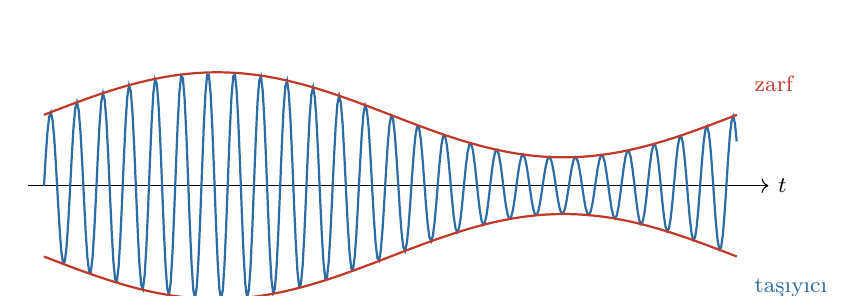
\begin{tikzpicture}[scale=1.0]
\draw[->] (-0.2,0)--(9.2,0) node[right]{\footnotesize $t$};
\draw[grafikMavi,thick,domain=0:8.8,samples=400]
  plot (\x,{(1+0.6*sin(deg(2*pi*\x/8.8)))*0.9*sin(deg(2*pi*\x*3))});
\draw[kirmizi,thick,domain=0:8.8,samples=200]
  plot (\x,{0.9*(1+0.6*sin(deg(2*pi*\x/8.8)))});
\draw[kirmizi,thick,domain=0:8.8,samples=200]
  plot (\x,{-0.9*(1+0.6*sin(deg(2*pi*\x/8.8)))});
\node[kirmizi,right] at (8.9,1.3) {\footnotesize zarf};
\node[grafikMavi,right] at (8.9,-1.3) {\footnotesize taşıyıcı};
\end{tikzpicture}
\end{center}

\gsub{AM Modülatörü}

\begin{lstlisting}
import numpy as np
from scipy import signal as sig

fs = 200_000                 # ornekleme
fc = 20_000                  # tasiyici
fm = 500                     # mesaj
m  = 0.7                     # modulasyon indeksi

t = np.arange(int(0.05*fs))/fs
mesaj = np.sin(2*np.pi*fm*t)
am = (1 + m*mesaj)*np.cos(2*np.pi*fc*t)

# Bant temeli karsiligi (IQ): faz sabit, genlik degisiyor
z_am = (1 + m*mesaj).astype(np.complex64)
\end{lstlisting}

\form[AM Verimliliği]{Toplam gücün taşıyıcıya giden kısmı bilgi taşımaz:
\[
\eta=\frac{m^2/2}{1+m^2/2}\Big|_{\text{sinüs mesaj}} ,
\]
$m=1$ için bile yalnızca $\%33$. Bu yüzden taşıyıcıyı ve bir yan bandı silen
\textbf{SSB} (tek yan bant) telsizde tercih edilir.}

\begin{lstlisting}
for m in [0.3, 0.5, 1.0]:
    eta = (m**2/2)/(1 + m**2/2)
    print(f"m={m:>4}  verim = {100*eta:5.1f} %")
# m= 0.3  verim =   4.3 %
# m= 0.5  verim =  11.1 %
# m= 1.0  verim =  33.3 %
\end{lstlisting}

\gsub{Zarf Detektörü ile Demodülasyon}

En basit AM demodülasyonu: analitik işaretin mutlak değeri (ya da donanımda
diyot + RC).

\begin{lstlisting}
def am_zarf_demod(s, fs, ses_kesim=5000):
    """Zarf detektoru: |analitik isaret| - DC."""
    zarf = np.abs(sig.hilbert(s))
    b = sig.firwin(129, ses_kesim, fs=fs)
    zarf = sig.lfilter(b, 1.0, zarf)
    return zarf - np.mean(zarf)                 # tasiyici DC'sini at

ses = am_zarf_demod(am, fs)
print(np.corrcoef(ses[200:], mesaj[200:])[0, 1])    # ~0.999
\end{lstlisting}

\begin{lstlisting}
# IQ akisindan geliyorsa daha da kolay:
def am_demod_iq(z, fs, ses_kesim=5000):
    zarf = np.abs(z)
    b = sig.firwin(129, ses_kesim, fs=fs)
    return sig.lfilter(b, 1.0, zarf - np.mean(zarf))
\end{lstlisting}

\gsub{Senkron (Coherent) Demodülasyon}

Zarf detektörü gürültüde zayıftır ve aşırı modülasyonda çalışmaz. Senkron
detektör taşıyıcıyı yeniden üretip çarpar; 3 dB daha iyi SNR verir.

\begin{lstlisting}
def am_senkron_demod(s, fs, fc, ses_kesim=5000):
    """Tasiyiciyi yeniden uretip carpma (faz kilitli olmali)."""
    n = np.arange(len(s))
    z = s*np.exp(-2j*np.pi*fc*n/fs)             # bant temeline indir
    b = sig.firwin(129, ses_kesim, fs=fs)
    z = sig.lfilter(b, 1.0, z)
    # Faz hatasini gider: isaretin ortalama fazina gore dondur
    z = z*np.exp(-1j*np.angle(np.mean(z)))
    return z.real - np.mean(z.real)
\end{lstlisting}

\uyari{Senkron demodülasyonda taşıyıcı fazı $\theta$ kadar kayarsa çıkış
$\cos\theta$ ile çarpılır: $\theta=90^\circ$'de \textbf{ses tamamen kaybolur}.
Bu yüzden gerçek alıcılarda faz, bir PLL veya Costas döngüsüyle kilitlenir
(bu kısmın sonunda).}

% =====================================================================
\gsec{FM: Frekans Modülasyonu}
% =====================================================================

\form[FM Denklemi]{
\[
s(t)=A_c\cos\Big(2\pi f_ct+2\pi k_f\!\int_0^t m(\tau)\dd\tau\Big),
\qquad
\Delta f=k_f\max|m|
\]
$\Delta f$ \textbf{frekans sapmasıdır} (FM radyoda 75 kHz). Modülasyon
indeksi $\beta=\Delta f/f_m$'dir.}

\form[Carson Kuralı]{FM işaretinin pratik bant genişliği:
\[
B\approx 2(\Delta f+f_{m,\max})=2f_{m,\max}(\beta+1).
\]
FM radyo için $2(75+15)=180$ kHz --- kanal aralığının neden 200 kHz olduğunun
cevabı.}

\gsub{Bessel: FM Spektrumu Neden Geniş?}

FM'in yan bantları Bessel fonksiyonlarıyla verilir:
\[
s(t)=A_c\sum_{n=-\infty}^{\infty}J_n(\beta)\cos\big(2\pi(f_c+nf_m)t\big).
\]

\begin{lstlisting}
from scipy.special import jv
import numpy as np

beta = 5.0
for n in range(8):
    print(f"J_{n}({beta}) = {jv(n, beta):+.4f}")

# Carson kurali dogrulamasi: gucun %98'ini kapsayan yan bant sayisi
guc = np.array([jv(n, beta)**2 for n in range(-40, 41)])
kum = np.cumsum(np.sort(guc)[::-1])/np.sum(guc)
print("gucun %98'i icin gereken bilesen:", np.searchsorted(kum, 0.98) + 1)
\end{lstlisting}

\begin{lstlisting}[style=outstyle]
J_0(5.0) = -0.1776
J_1(5.0) = -0.3276
J_2(5.0) = +0.0466
J_3(5.0) = +0.3648
J_4(5.0) = +0.3912
J_5(5.0) = +0.2611
J_6(5.0) = +0.1310
J_7(5.0) = +0.0534
\end{lstlisting}

\bilgi{$J_0(\beta)=0$ olduğu $\beta$ değerlerinde (2,405, 5,520, \dots)
taşıyıcı tamamen kaybolur. Laboratuvarda frekans sapmasını ölçmenin klasik
yolu budur: modülasyonu artırıp taşıyıcının söndüğü noktayı bulursun.}

\gsub{FM Modülatörü}

\begin{lstlisting}
import numpy as np

def fm_modulate(mesaj, fs, sapma_hz):
    """Bant temeli FM: faz = 2*pi*sapma*kumulatif(mesaj)/fs."""
    mesaj = mesaj/np.max(np.abs(mesaj))            # -1..1 normalize
    faz = 2*np.pi*sapma_hz*np.cumsum(mesaj)/fs
    return np.exp(1j*faz).astype(np.complex64)

fs = 240_000
t = np.arange(int(0.2*fs))/fs
ses = np.sin(2*np.pi*1000*t)
z_fm = fm_modulate(ses, fs, sapma_hz=75_000)
\end{lstlisting}

\uyari{\code{np.cumsum} tam olarak integralin ayrık karşılığıdır ama uzun
dizilerde \code{float32} ile birikimli yuvarlama hatası yapar; faz için
\code{float64} kullan, sonucu \code{complex64}'e çevir.}

\gsub{FM Demodülasyonu: IQ Diskriminatör}

FM demodülasyonu tek satırdır: ardışık örneklerin \emph{faz farkı}, anlık
frekansla orantılıdır.

\form[Polar Diskriminatör]{
\[
\hat{m}[n]=\arg\big(z[n]\,z^*[n-1]\big)\cdot\frac{f_s}{2\pi\Delta f}
\]
Çarpım $z[n]z^*[n-1]$, iki fazör arasındaki açı farkını verir; \code{np.angle}
bunu $[-\pi,\pi]$ aralığında güvenle döndürür (faz sarması sorunu yok).}

\begin{lstlisting}
import numpy as np

def fm_demod(z, fs=None, sapma_hz=None):
    """IQ polar diskriminator. Olcekleme istege bagli."""
    d = np.angle(z[1:]*np.conj(z[:-1]))
    if fs and sapma_hz:
        d = d*fs/(2*np.pi*sapma_hz)
    return d

geri = fm_demod(z_fm, fs, 75_000)
print(np.corrcoef(geri[100:], ses[101:])[0, 1])     # ~0.9999
\end{lstlisting}

\ipucu{\code{np.angle(z[1:]*conj(z[:-1]))} yerine
\code{np.diff(np.unwrap(np.angle(z)))} de aynı sonucu verir ama daha
yavaştır ve gürültüde \code{unwrap} hata yapabilir. Çarpım yöntemi hem hızlı
hem sağlamdır --- SDR alıcılarının standardıdır.}

\gsub{De-emphasis: FM'in Son Rötuşu}

Vericide yüksek frekanslar yükseltilir (pre-emphasis), alıcıda aynı oranda
bastırılır (de-emphasis); böylece FM'in yüksek frekanslarda artan gürültüsü
azalır. Zaman sabiti Avrupa'da $50\ \mu$s, ABD'de $75\ \mu$s'tir.

\begin{lstlisting}
from scipy import signal as sig

def deemphasis(x, fs, tau=50e-6):
    """Tek kutuplu RC alcak gecirgen (bilinear donusum ile)."""
    # H(s) = 1/(1 + s*tau)  ->  sayisal karsiligi
    b, a = sig.bilinear([1.0], [tau, 1.0], fs=fs)
    return sig.lfilter(b, a, x)
\end{lstlisting}

\ornek{De-emphasis unutulursa FM radyo ``tiz ve cızırtılı'' duyulur; yanlış
zaman sabiti kullanılırsa ses boğuk veya keskin olur. Bu, ev yapımı SDR
alıcılarında en sık atlanan adımdır.}

% =====================================================================
\gsec{PM: Faz Modülasyonu}
% =====================================================================

\form{
\[
s(t)=A_c\cos\big(2\pi f_ct+k_p m(t)\big)
\]
FM ile PM kardeştir: $m(t)$'nin integralini alıp PM uygularsan FM elde
edersin. Bu yüzden pratikte tek bir IQ modülatör ikisini de üretir.}

\begin{lstlisting}
def pm_modulate(mesaj, k_p=1.0):
    return np.exp(1j*k_p*mesaj).astype(np.complex64)

def pm_demod(z):
    return np.unwrap(np.angle(z))

# FM ile PM iliskisi
z_pm_of_integral = pm_modulate(np.cumsum(ses)*2*np.pi*75_000/fs)
print(np.allclose(z_pm_of_integral, fm_modulate(ses, fs, 75_000), atol=1e-5))
\end{lstlisting}

% =====================================================================
\gsec{Sayısal Modülasyonlar: ASK, FSK, PSK, QAM}
% =====================================================================

Sayısal modülasyonda bilgi \emph{sürekli} değil, sonlu bir sembol kümesinden
seçilir. Her sembol $\log_2 M$ bit taşır.

\begin{center}
\begin{tabularx}{\textwidth}{@{}>{\bfseries\color{anaMavi}}l c c >{\raggedright\arraybackslash}X@{}}
\toprule
\rowcolor{acikMavi}\multicolumn{1}{@{}l}{\color{anaMavi}\textbf{Şema}} & \multicolumn{1}{c}{\color{anaMavi}\textbf{bit/sembol}} & \multicolumn{1}{c}{\color{anaMavi}\textbf{$E_b/N_0$ @ $10^{-3}$}} & \multicolumn{1}{l@{}}{\color{anaMavi}\textbf{Not}}\\
\midrule
BPSK & 1 & 6,8 dB & En dayanıklı; uzay haberleşmesi.\\
\rowcolor{acikGri} QPSK & 2 & 6,8 dB & BPSK ile aynı BER, iki kat hız.\\
8-PSK & 3 & 10,0 dB & Faz aralığı daralır, gürültüye duyarlı.\\
\rowcolor{acikGri} 16-QAM & 4 & 10,5 dB & Genlik + faz; doğrusal yükselteç ister.\\
64-QAM & 6 & 14,8 dB & Yüksek SNR gerektirir (Wi-Fi, LTE).\\
\bottomrule
\end{tabularx}
\end{center}

\gsub{BPSK ve QPSK}

\begin{lstlisting}
import numpy as np

rng = np.random.default_rng(0)
bitler = rng.integers(0, 2, 10_000)

# BPSK: 0 -> -1,  1 -> +1
bpsk = (2*bitler - 1).astype(np.complex64)

# QPSK (Gray kodlu): bit ciftleri -> 4 faz
b2 = bitler.reshape(-1, 2)
qpsk = ((1 - 2*b2[:, 0]) + 1j*(1 - 2*b2[:, 1]))/np.sqrt(2)

print(np.mean(np.abs(qpsk)**2))       # 1.0  -> birim ortalama guc
\end{lstlisting}

\form[Gray Kodlama]{Komşu takımyıldız noktaları yalnızca \emph{tek bitte}
farklı olacak şekilde eşlenirse, en sık görülen hata (komşuya kayma) tek bit
hatası üretir. Bu, aynı SNR'de bit hata oranını yaklaşık yarıya indirir ---
bedelsiz bir kazanç.}

\gsub{FSK}

\begin{lstlisting}
def fsk_modulate(bitler, fs, sembol_hizi, ayirma_hz):
    """Surekli fazli FSK (CPFSK): faz sicramasi yok."""
    sps = int(fs/sembol_hizi)                       # sembol basina ornek
    frek = np.where(bitler > 0, ayirma_hz/2, -ayirma_hz/2)
    frek = np.repeat(frek, sps)
    faz = 2*np.pi*np.cumsum(frek)/fs
    return np.exp(1j*faz).astype(np.complex64)

def fsk_demod(z, fs, sembol_hizi, ayirma_hz):
    d = np.angle(z[1:]*np.conj(z[:-1]))*fs/(2*np.pi)   # anlik frekans (Hz)
    sps = int(fs/sembol_hizi)
    d = d[:len(d)//sps*sps].reshape(-1, sps).mean(axis=1)
    return (d > 0).astype(int)
\end{lstlisting}

\bilgi{Sürekli fazlı FSK (CPFSK) faz sıçraması içermediği için spektrumu
dardır. Gauss filtresiyle yumuşatılmış hâli \textbf{GFSK}'dır ve Bluetooth
ile birçok IoT telsizinin modülasyonudur.}

\gsub{QAM}

\begin{lstlisting}
def qam_takimyildiz(M):
    """Kare M-QAM takimyildizi (birim ortalama guce normalize)."""
    k = int(np.sqrt(M))
    seviye = np.arange(-(k-1), k, 2)
    I, Q = np.meshgrid(seviye, seviye)
    c = (I + 1j*Q).ravel()
    return c/np.sqrt(np.mean(np.abs(c)**2))

c16 = qam_takimyildiz(16)
print(len(c16), np.mean(np.abs(c16)**2))     # 16 1.0

def qam_karar(z, takim):
    """En yakin komsu karari (hard decision)."""
    d = np.abs(z[:, None] - takim[None, :])
    return np.argmin(d, axis=1)
\end{lstlisting}

\uyari{QAM genlik bilgisi taşıdığı için vericinin güç yükselteci
\emph{doğrusal} olmalıdır; FM/FSK'de kullanılan verimli doyumlu (class-C)
yükselteçler QAM'i bozar. Bu, 5G baz istasyonlarının neden pahalı doğrusal
yükselteç kullandığının cevabıdır.}

% =====================================================================
\gsec{Darbe Şekillendirme ve Göz Diyagramı}
% =====================================================================

Sembolleri kare darbelerle göndermek spektrumu sonsuz genişletir. Çözüm,
darbeleri şekillendirmektir --- ama şekil, komşu sembollere sızmamalıdır.

\form[Nyquist ISI Kriteri]{Bir darbe, sembol anlarında ($t=kT$, $k\neq0$)
sıfır oluyorsa \textbf{semboller arası girişim (ISI)} üretmez. \emph{Raised
cosine} ailesi bu koşulu sağlar; $\beta$ (roll-off) bant genişliğini
$(1+\beta)/2T$ yapar.}

\begin{lstlisting}
import numpy as np

def rrc(beta, sps, span=10):
    """Kok yukseltilmis kosinus (root raised cosine) darbesi."""
    N = span*sps
    t = (np.arange(N + 1) - N/2)/sps
    h = np.zeros_like(t)
    for i, ti in enumerate(t):
        if np.isclose(ti, 0.0):
            h[i] = 1 - beta + 4*beta/np.pi
        elif beta > 0 and np.isclose(abs(ti), 1/(4*beta)):
            h[i] = (beta/np.sqrt(2))*((1 + 2/np.pi)*np.sin(np.pi/(4*beta))
                                      + (1 - 2/np.pi)*np.cos(np.pi/(4*beta)))
        else:
            pay = (np.sin(np.pi*ti*(1 - beta))
                   + 4*beta*ti*np.cos(np.pi*ti*(1 + beta)))
            payda = np.pi*ti*(1 - (4*beta*ti)**2)
            h[i] = pay/payda
    return h/np.sqrt(np.sum(h**2))

sps, beta = 8, 0.35
h = rrc(beta, sps)

# Vericide sekillendirme: sembolleri sps kat yukari orneklendir, filtrele
semboller = qpsk
yukari = np.zeros(len(semboller)*sps, dtype=complex)
yukari[::sps] = semboller
tx = np.convolve(yukari, h, mode='same')
\end{lstlisting}

\bilgi{Kök yükseltilmiş kosinüs vericide \emph{ve} alıcıda uygulanır; ikisinin
çarpımı tam yükseltilmiş kosinüs olur ve ISI sıfırlanır. Buna \emph{eşlenik
filtre} (matched filter) denir ve aynı zamanda SNR'yi maksimize eder ---
iki kazanç bir arada.}

\gsub{Göz Diyagramı}

\begin{lstlisting}
import matplotlib.pyplot as plt

def goz_diyagrami(x, sps, n_iz=200, baslik=''):
    """Ardisik 2 sembolluk parcalari ust uste cizer."""
    x = np.real(x)
    L = 2*sps
    plt.figure(figsize=(6, 4))
    for i in range(n_iz):
        p = x[i*sps:i*sps + L]
        if len(p) == L:
            plt.plot(np.arange(L)/sps, p, color='#2E6DA4', alpha=0.15, lw=0.8)
    plt.grid(alpha=0.3); plt.xlabel('Sembol'); plt.title(baslik); plt.show()

goz_diyagrami(np.convolve(tx, h, mode='same'), sps, baslik='RRC x RRC (ISI yok)')
\end{lstlisting}

\ornek{Göz diyagramı okuma: \emph{gözün açıklığı} gürültü payını, \emph{dikey
kalınlık} genlik bozulmasını, \emph{yatay bulanıklık} zamanlama titreşimini
(jitter) gösterir. Göz kapanmışsa ya ISI ya da SNR sorunu vardır.}

% =====================================================================
\gsec{Taşıyıcı ve Zamanlama Kurtarma}
% =====================================================================

Alıcı, vericinin ne fazını ne de sembol saatini bilir. İki döngü bunu
düzeltir: \textbf{taşıyıcı kurtarma} (faz/frekans) ve \textbf{zamanlama
kurtarma} (örnekleme anı).

\gsub{Faz Kilitlemeli Döngü (PLL)}

\begin{center}
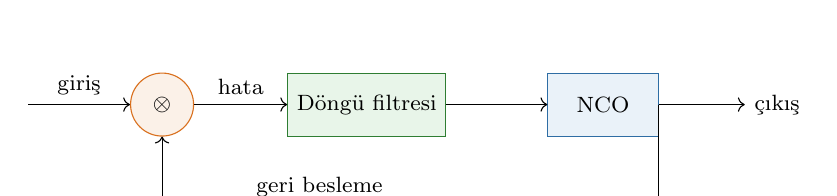
\begin{tikzpicture}[scale=1.0, every node/.style={font=\footnotesize}]
\node[draw=turuncu,fill=turuncu!10,circle,minimum size=0.8cm] (pd) at (0,0) {$\otimes$};
\node[draw=yesil,fill=acikYesil,minimum width=1.6cm,minimum height=0.8cm] (lf) at (2.6,0) {Döngü filtresi};
\node[draw=vurguMavi,fill=acikMavi,minimum width=1.4cm,minimum height=0.8cm] (nco) at (5.6,0) {NCO};
\draw[->] (-1.7,0)--(pd) node[midway,above] {giriş};
\draw[->] (pd)--(lf) node[midway,above] {hata};
\draw[->] (lf)--(nco);
\draw[->] (nco)--(7.4,0) node[right] {çıkış};
\draw[->] (6.3,0)--(6.3,-1.2)--(0,-1.2)--(pd) node[midway,below,xshift=2cm] {geri besleme};
\end{tikzpicture}
\end{center}

\begin{lstlisting}
import numpy as np

def pll(z, bant=0.01, zeta=0.707):
    """Ikinci mertebe PLL: tasiyici faz/frekans ofsetini duzeltir."""
    # Doner Gardner/Rice katsayilari
    Kp = 4*zeta*bant/(1 + 2*zeta*bant + bant**2)
    Ki = 4*bant**2/(1 + 2*zeta*bant + bant**2)

    faz, frek = 0.0, 0.0
    cikis = np.empty_like(z)
    for n in range(len(z)):
        y = z[n]*np.exp(-1j*faz)
        cikis[n] = y
        hata = np.angle(y)                 # basit faz dedektoru
        frek += Ki*hata
        faz  += frek + Kp*hata
    return cikis
\end{lstlisting}

\uyari{Bu döngü örnek başına Python yorumlayıcısında çalışır: 1 M örnek için
saniyeler sürer. Gerçek kullanımda \code{numba.njit} ile derle
(\code{@njit} eklemek 50--100 kat hızlandırır) veya bloklu kestirim
kullan.}

\gsub{Costas Döngüsü: PSK için Taşıyıcı Kurtarma}

BPSK/QPSK'da veri fazı $180^\circ$/$90^\circ$ atladığı için düz PLL kilitlenmez.
Costas döngüsü, veri modülasyonunu kaldıran bir faz dedektörü kullanır.

\begin{lstlisting}
def costas_qpsk(z, bant=0.005, zeta=0.707):
    Kp = 4*zeta*bant/(1 + 2*zeta*bant + bant**2)
    Ki = 4*bant**2/(1 + 2*zeta*bant + bant**2)
    faz, frek = 0.0, 0.0
    y = np.empty_like(z)
    for n in range(len(z)):
        v = z[n]*np.exp(-1j*faz)
        y[n] = v
        # QPSK faz dedektoru: karar yonlu (decision-directed)
        hata = (np.sign(v.real)*v.imag - np.sign(v.imag)*v.real)
        frek += Ki*hata
        faz  += frek + Kp*hata
    return y
\end{lstlisting}

\bilgi{BPSK için faz dedektörü daha da basittir:
\code{hata = v.real*v.imag}. Costas döngüsünün $180^\circ$ (QPSK'da
$90^\circ$) belirsizliği vardır: doğru kilitlenir ama hangi faza kilitlendiği
bilinmez. Çözüm, \emph{diferansiyel kodlama} ya da bilinen bir başlık
(preamble) kullanmaktır.}

\gsub{Sembol Zamanlama Kurtarma: Gardner}

\begin{lstlisting}
def gardner_tzk(z, sps, kazanc=0.05):
    """Gardner zamanlama hata dedektoru ile sembol ortasina kilitleme."""
    mu = 0.0                       # kesirli gecikme
    i = sps
    cikis = []
    while i + sps < len(z):
        idx = int(i)
        simdi = z[idx]
        orta  = z[idx - sps//2]
        onceki = z[idx - sps]
        # Gardner hatasi: genlikten bagimsiz, tasiyici fazina duyarsiz
        hata = (np.real(orta)*(np.real(simdi) - np.real(onceki))
                + np.imag(orta)*(np.imag(simdi) - np.imag(onceki)))
        mu += kazanc*hata
        i  += sps + mu
        cikis.append(simdi)
    return np.array(cikis)
\end{lstlisting}

\ipucu{Gardner dedektörünün en güzel yanı, taşıyıcı fazı henüz
kilitlenmemişken bile çalışmasıdır. Bu yüzden tipik alıcı sırası şudur:
AGC $\to$ eşlenik filtre $\to$ zamanlama kurtarma $\to$ taşıyıcı kurtarma
$\to$ karar. Kısım 7'deki QPSK modeminde bu zinciri baştan sona kuracağız.}

% #####################################################################
\gpart{6}{Uçtan Uca: Tam Bir FM Radyo Alıcısı}
% #####################################################################

% =====================================================================
\gsec{IQ Dosya Formatları ve RTL-SDR}
% =====================================================================

SDR donanımları IQ örneklerini birkaç standart formatta verir. Doğru
yorumlamak, alıcının ilk ve en kritik adımıdır.

\begin{center}
\begin{tabularx}{\textwidth}{@{}>{\bfseries\color{anaMavi}}l >{\ttfamily}l >{\raggedright\arraybackslash}X@{}}
\toprule
\rowcolor{acikMavi}\multicolumn{1}{@{}l}{\color{anaMavi}\textbf{Format}} & \multicolumn{1}{l}{\color{anaMavi}\textbf{dtype}} & \multicolumn{1}{l@{}}{\color{anaMavi}\textbf{Nerede?}}\\
\midrule
cu8 & uint8 & RTL-SDR ham çıktısı; merkez 127,5.\\
\rowcolor{acikGri} cs8 & int8 & HackRF.\\
cs16 & int16 & Airspy, SDRplay, birçok kayıt dosyası.\\
\rowcolor{acikGri} cf32 & complex64 & GNU Radio standardı; işlemede kullanılan tip.\\
\bottomrule
\end{tabularx}
\end{center}

\begin{lstlisting}
import numpy as np

def cu8_oku(dosya, sayi=-1, ofset=0):
    """RTL-SDR ham (uint8, I/Q sirali) dosyasini complex64'e cevirir."""
    ham = np.fromfile(dosya, dtype=np.uint8,
                      count=-1 if sayi < 0 else 2*sayi, offset=2*ofset)
    ham = ham.astype(np.float32)
    ham = (ham - 127.5)/127.5                 # -1..1 araligina getir
    return (ham[0::2] + 1j*ham[1::2]).astype(np.complex64)

def cf32_oku(dosya):
    return np.fromfile(dosya, dtype=np.complex64)

def cs16_oku(dosya):
    ham = np.fromfile(dosya, dtype=np.int16).astype(np.float32)/32768.0
    return (ham[0::2] + 1j*ham[1::2]).astype(np.complex64)
\end{lstlisting}

\uyari{En sık yapılan hata I/Q sırasını ters almaktır. Sonuç: spektrum aynaya
düşer, FM sesi ``tersine'' çıkar. Şüphelenirsen \code{np.conj(iq)} deneyerek
kontrol et --- doğru olan, istasyonun beklenen frekansta görünmesidir.}

\gsub{Donanımdan Canlı Akış}

\begin{lstlisting}
from rtlsdr import RtlSdr
import numpy as np

sdr = RtlSdr()
sdr.sample_rate = 2.4e6            # 2.4 MS/s
sdr.center_freq = 100.1e6          # istasyon frekansi
sdr.freq_correction = 60           # ppm duzeltmesi
sdr.gain = 'auto'

iq = sdr.read_samples(256*1024)    # complex128 doner
iq = iq.astype(np.complex64)
sdr.close()

# Surekli akis (async)
def kare_isle(ornekler, ctx):
    ses = wbfm_al(ornekler.astype(np.complex64))
    ...                              # ses cikisina yaz

# sdr.read_samples_async(kare_isle, 256*1024)
\end{lstlisting}

\bilgi{RTL-SDR'ın kristali tipik olarak 20--60 ppm kayar; 100 MHz'te bu
2--6 kHz'lik bir frekans hatası demektir. Geniş bant FM'de fark edilmez ama
dar bant (NFM, SSB, sayısal) modlarda \code{freq\_correction} ayarlanmazsa
demodülasyon bozulur.}

% =====================================================================
\gsec{Tam WBFM Alıcı Hattı}
% =====================================================================

Geniş bant FM (WBFM) alıcısı altı adımdır. Hepsi bu rehberde tek tek
işlendi; şimdi birleştiriyoruz.

\begin{center}
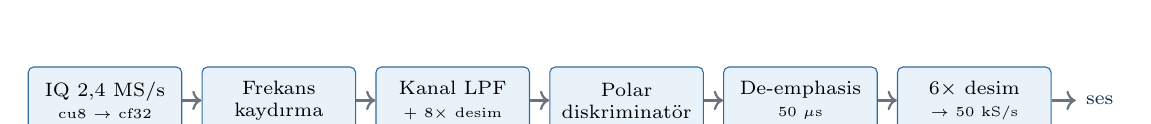
\begin{tikzpicture}[scale=0.92, every node/.style={font=\scriptsize},
  kutu/.style={draw=vurguMavi,fill=acikMavi,rounded corners=2pt,
               minimum width=1.95cm,minimum height=0.85cm,align=center}]
\node[kutu] (a) at (0,0) {IQ 2,4 MS/s\\ \tiny cu8 $\to$ cf32};
\node[kutu] (b) at (2.4,0) {Frekans\\kaydırma};
\node[kutu] (c) at (4.8,0) {Kanal LPF\\ \tiny + 8$\times$ desim};
\node[kutu] (d) at (7.2,0) {Polar\\diskriminatör};
\node[kutu] (e) at (9.6,0) {De-emphasis\\ \tiny 50 $\mu$s};
\node[kutu] (f) at (12.0,0) {6$\times$ desim\\ \tiny $\to$ 50 kS/s};
\foreach \x/\y in {a/b, b/c, c/d, d/e, e/f} \draw[->,thick,ortaGri] (\x)--(\y);
\draw[->,thick,ortaGri] (f)--(13.4,0) node[right,anaMavi,font=\scriptsize] {ses};
\end{tikzpicture}
\end{center}

\begin{lstlisting}
import numpy as np
from scipy import signal as sig
import soundfile as sf


class WBFMAlici:
    """RTL-SDR IQ akisindan ses ureten tam FM alicisi."""

    def __init__(self, fs_in=2_400_000, kanal_ofset=0.0,
                 fs_ara=240_000, fs_ses=48_000, tau=50e-6):
        self.fs_in = fs_in
        self.ofset = kanal_ofset
        self.dec1 = int(fs_in//fs_ara)             # 10
        self.fs_ara = fs_in//self.dec1
        self.dec2 = int(self.fs_ara//fs_ses)       # 5
        self.fs_ses = self.fs_ara//self.dec2

        # Kanal filtresi: WBFM icin +-100 kHz
        self.h_kanal = sig.firwin(129, 100_000, fs=fs_in).astype(np.float32)
        # Ses filtresi: 15 kHz'e kadar
        self.h_ses = sig.firwin(129, 15_000, fs=self.fs_ara).astype(np.float32)
        # De-emphasis
        self.b_de, self.a_de = sig.bilinear([1.0], [tau, 1.0], fs=self.fs_ara)

        # Bloklar arasi durumlar
        self.zi_kanal = np.zeros(len(self.h_kanal) - 1, dtype=np.complex64)
        self.zi_ses = np.zeros(len(self.h_ses) - 1, dtype=np.float32)
        self.zi_de = np.zeros(max(len(self.a_de), len(self.b_de)) - 1)
        self.faz = 0.0
        self.son_ornek = np.complex64(1.0)

    def _kaydir(self, z):
        n = np.arange(len(z))
        adim = 2*np.pi*(-self.ofset)/self.fs_in
        lo = np.exp(1j*(self.faz + adim*n)).astype(np.complex64)
        self.faz = (self.faz + adim*len(z)) % (2*np.pi)
        return z*lo

    def isle(self, iq):
        z = iq.astype(np.complex64)
        if self.ofset:
            z = self._kaydir(z)

        # 1) Kanal filtresi + desimasyon
        z, self.zi_kanal = sig.lfilter(self.h_kanal, 1.0, z, zi=self.zi_kanal)
        z = z[::self.dec1]

        # 2) Polar diskriminator (blok sinirinda faz surekliligi icin
        #    onceki blogun son ornegini basa ekliyoruz)
        z = np.concatenate(([self.son_ornek], z))
        self.son_ornek = z[-1]
        ses = np.angle(z[1:]*np.conj(z[:-1])).astype(np.float32)

        # 3) De-emphasis
        ses, self.zi_de = sig.lfilter(self.b_de, self.a_de, ses, zi=self.zi_de)

        # 4) Ses bandi filtresi + desimasyon
        ses, self.zi_ses = sig.lfilter(self.h_ses, 1.0, ses, zi=self.zi_ses)
        ses = ses[::self.dec2]

        # 5) Normalize
        return (ses/(np.max(np.abs(ses)) + 1e-9)*0.7).astype(np.float32)


# Kullanim: kayitli bir dosyadan
alici = WBFMAlici(fs_in=2_400_000, kanal_ofset=0.0)
iq = cu8_oku('kayit_100M1.iq')
ses = np.concatenate([alici.isle(iq[i:i+262144])
                      for i in range(0, len(iq), 262144)])
sf.write('radyo.wav', ses, alici.fs_ses)
print(f"{len(ses)/alici.fs_ses:.1f} saniye ses uretildi @ {alici.fs_ses} Hz")
\end{lstlisting}

\uyari{Blok blok işlerken üç şeyin durumu taşınmalıdır: (1) FIR/IIR filtre
durumları (\code{zi}), (2) NCO fazı, (3) diskriminatörün bir önceki örneği.
Üçü de yukarıdaki sınıfta saklanıyor. Biri unutulursa her blok sınırında
duyulabilir bir ``tık'' oluşur.}

\gsub{Dar Bant FM (NFM) Farkı}

\begin{center}
\begin{tabularx}{\textwidth}{@{}>{\bfseries\color{anaMavi}}l c c >{\raggedright\arraybackslash}X@{}}
\toprule
\rowcolor{acikMavi}\multicolumn{1}{@{}l}{\color{anaMavi}\textbf{Parametre}} & \multicolumn{1}{c}{\color{anaMavi}\textbf{WBFM}} & \multicolumn{1}{c}{\color{anaMavi}\textbf{NFM}} & \multicolumn{1}{l@{}}{\color{anaMavi}\textbf{Not}}\\
\midrule
Sapma & 75 kHz & 2,5--5 kHz & NFM telsizlerde.\\
\rowcolor{acikGri} Kanal filtresi & 100 kHz & 6--8 kHz & Dar filtre $\to$ daha uzun FIR.\\
Ses bandı & 15 kHz & 3 kHz & Konuşma yeterli.\\
\rowcolor{acikGri} De-emphasis & 50/75 $\mu$s & 750 $\mu$s & Ya da hiç.\\
\bottomrule
\end{tabularx}
\end{center}

\begin{lstlisting}
# NFM icin ayni sinif, farkli parametreler
nfm = WBFMAlici(fs_in=2_400_000, fs_ara=48_000, fs_ses=48_000, tau=750e-6)
nfm.h_kanal = sig.firwin(301, 8_000, fs=2_400_000).astype(np.float32)
\end{lstlisting}

% =====================================================================
\gsec{Performans ve Gerçek Zamanlı Akış}
% =====================================================================

\gsub{Ne Kadar Hızlı Olmalı?}

2,4 MS/s'lik bir akışı gerçek zamanlı işlemek için saniyede 2,4 milyon
karmaşık örneği yetiştirmek gerekir. Doğru yazılmış NumPy kodu bunu rahatlıkla
yapar; yanlış yazılmış Python döngüsü asla yapamaz.

\begin{center}
\begin{tabularx}{\textwidth}{@{}>{\bfseries\color{anaMavi}}l >{\raggedright\arraybackslash}X@{}}
\toprule
\rowcolor{acikMavi}\multicolumn{1}{@{}l}{\color{anaMavi}\textbf{Teknik}} & \multicolumn{1}{l@{}}{\color{anaMavi}\textbf{Kazanç}}\\
\midrule
Erken desimasyon & En pahalı işlemleri en düşük hızda yap. Tek başına 10--50 kat.\\
\rowcolor{acikGri} \code{complex64} kullan & Bellek yarı, FFT $\sim$1,7 kat hızlı.\\
\code{resample\_poly} & Polifaz, saf filtre+desimasyona göre $M$ kat az çarpma.\\
\rowcolor{acikGri} \code{sig.lfilter}/\code{sosfilt} & C uygulaması; Python döngüsünden 100+ kat hızlı.\\
\code{numba.njit} & Kaçınılmaz örnek-bazlı döngüler (PLL, Viterbi) için 50--100 kat.\\
\rowcolor{acikGri} \code{scipy.fft(workers=-1)} & Çok çekirdekli FFT.\\
Önceden ayrılmış tampon & \code{np.empty} + \code{out=} ile blok başına ayırma yapma.\\
\bottomrule
\end{tabularx}
\end{center}

\begin{lstlisting}
# Darbogazi olcmeden optimize etme
import cProfile, pstats

cProfile.run('alici.isle(iq[:262144])', 'prof.out')
pstats.Stats('prof.out').sort_stats('cumulative').print_stats(10)
\end{lstlisting}

\gsub{Üretici--Tüketici ile Gerçek Zamanlı Alıcı}

\begin{lstlisting}
import queue, threading
import numpy as np, sounddevice as sd
from rtlsdr import RtlSdr

kuyruk = queue.Queue(maxsize=8)
alici = WBFMAlici()

def sdr_okuyucu():
    sdr = RtlSdr()
    sdr.sample_rate, sdr.center_freq, sdr.gain = 2.4e6, 100.1e6, 'auto'
    try:
        while calisiyor:
            blok = sdr.read_samples(262144).astype(np.complex64)
            try:
                kuyruk.put_nowait(blok)
            except queue.Full:
                pass                     # gec kalan blogu at (drop)
    finally:
        sdr.close()

def ses_callback(outdata, frames, time, status):
    global tampon
    while len(tampon) < frames:
        tampon = np.concatenate([tampon, alici.isle(kuyruk.get())])
    outdata[:, 0] = tampon[:frames]
    tampon = tampon[frames:]

calisiyor, tampon = True, np.zeros(0, dtype=np.float32)
threading.Thread(target=sdr_okuyucu, daemon=True).start()
with sd.OutputStream(samplerate=alici.fs_ses, channels=1,
                     blocksize=2048, callback=ses_callback):
    sd.sleep(60_000)
calisiyor = False
\end{lstlisting}

\uyari{Kuyruk dolduğunda bloğu \emph{atmak}, beklemekten iyidir: radyo canlı
bir akıştır, gecikmiş veri işe yaramaz. Kuyruk sürekli doluyorsa işleme
hattın gerçek zamandan yavaş demektir --- desimasyonu öne al veya filtre
uzunluğunu kısalt.}

\gsub{Nereye Bakmalı?}

\begin{center}
\begin{tabularx}{\textwidth}{@{}>{\bfseries\color{anaMavi}}l >{\raggedright\arraybackslash}X@{}}
\toprule
\rowcolor{acikMavi}\multicolumn{1}{@{}l}{\color{anaMavi}\textbf{Kaynak}} & \multicolumn{1}{l@{}}{\color{anaMavi}\textbf{Ne için?}}\\
\midrule
GNU Radio & Grafik akış tabanlı SDR çerçevesi; Python blokları yazılabilir.\\
\rowcolor{acikGri} SoapySDR & Donanımdan bağımsız sürücü katmanı (RTL, HackRF, USRP\dots).\\
PySDR (pysdr.org) & Python odaklı, ücretsiz ve çok iyi bir DSP/SDR kitabı.\\
\rowcolor{acikGri} scipy.signal belgeleri & Filtre tasarımı ve spektral analizin başvuru kaynağı.\\
Lyons, \emph{Understanding DSP} & Sezgisel anlatımıyla klasik DSP kitabı.\\
\bottomrule
\end{tabularx}
\end{center}

% #####################################################################
\gpart{7}{İleri Konular}
% #####################################################################

% =====================================================================
\gsec{Stereo FM Çözücü}
% =====================================================================

FM yayınının bant temeli işareti (\emph{multiplex}, MPX) birden çok bilgiyi
frekansta ayırarak taşır:

\begin{center}
\begin{tabularx}{\textwidth}{@{}>{\bfseries\color{anaMavi}}l >{\raggedright\arraybackslash}X@{}}
\toprule
\rowcolor{acikMavi}\multicolumn{1}{@{}l}{\color{anaMavi}\textbf{Bant}} & \multicolumn{1}{l@{}}{\color{anaMavi}\textbf{İçerik}}\\
\midrule
0--15 kHz & $L+R$ (mono uyumluluk için).\\
\rowcolor{acikGri} 19 kHz & Pilot ton (stereo göstergesi ve faz referansı).\\
23--53 kHz & $L-R$, 38 kHz'te DSB-SC (bastırılmış taşıyıcı).\\
\rowcolor{acikGri} 57 kHz & RDS/RBDS veri (1187,5 bps).\\
67/92 kHz & SCA (abonelik yayınları).\\
\bottomrule
\end{tabularx}
\end{center}

\form[Stereo Matris]{Pilotun \emph{ikinci harmoniği} (38 kHz) ile
$L-R$ bandını çarpıp alçak geçirirsek:
\[
L=(L+R)+(L-R),\qquad R=(L+R)-(L-R).
\]}

\begin{lstlisting}
import numpy as np
from scipy import signal as sig

def fm_stereo_coz(mpx, fs_mpx, fs_ses=48_000):
    """MPX isaretinden (diskriminator cikisi) L ve R kanallarini uretir."""
    # 1) Mono: L+R  (0-15 kHz)
    h_mono = sig.firwin(257, 15_000, fs=fs_mpx)
    lr_toplam = sig.lfilter(h_mono, 1.0, mpx)

    # 2) Pilot: 19 kHz dar bant geciren
    sos_pilot = sig.butter(4, [18_800, 19_200], btype='bandpass',
                           fs=fs_mpx, output='sos')
    pilot = sig.sosfiltfilt(sos_pilot, mpx)

    # 3) Pilotun 2. harmonigini uret: analitik isaretin karesi
    pilot_a = sig.hilbert(pilot)
    tasiyici38 = np.real(pilot_a**2/(np.abs(pilot_a)**2 + 1e-12))   # cos(2*w*t)

    # 4) L-R bandini asagi cek ve alcak gecir
    sos_lr = sig.butter(6, [23_000, 53_000], btype='bandpass',
                        fs=fs_mpx, output='sos')
    lr_fark = sig.sosfiltfilt(sos_lr, mpx)*tasiyici38*2.0
    lr_fark = sig.lfilter(h_mono, 1.0, lr_fark)

    # 5) Matris ve ses hizina indirme
    L = lr_toplam + lr_fark
    R = lr_toplam - lr_fark
    M = int(fs_mpx//fs_ses)
    return sig.resample_poly(L, 1, M), sig.resample_poly(R, 1, M)


def stereo_var_mi(mpx, fs_mpx, esik_db=-30):
    """19 kHz pilotun varligina bakarak stereo olup olmadigini soyler."""
    N = min(len(mpx), 1 << 16)
    X = np.abs(np.fft.rfft(mpx[:N]*np.hanning(N)))
    f = np.fft.rfftfreq(N, 1/fs_mpx)
    k19 = np.argmin(np.abs(f - 19_000))
    seviye = 20*np.log10(X[k19]/np.max(X) + 1e-12)
    return seviye > esik_db, seviye
\end{lstlisting}

\uyari{Stereo çözmek için MPX işaretini \textbf{en az 100--120 kS/s} hızda
tutmalısın: 53 kHz'lik bileşeni koruman gerekir. WBFM alıcısında ara hızı
240 kS/s'te bırakıp stereo matristen \emph{sonra} 48 kS/s'e in.}

\bilgi{Pilotun karesini almak yerine faz kilitli bir PLL ile 38 kHz üretmek
gürültüde daha sağlamdır: pilot zayıfladığında karesi alma yöntemi gürültüyü
de kareler ve kanal ayrımı (separation) düşer.}

% =====================================================================
\gsec{Otomatik Kazanç Kontrolü (AGC)}
% =====================================================================

Alınan işaret seviyesi saniyeler içinde 40 dB değişebilir. AGC, çıkışı sabit
bir seviyeye getirir; demodülatörlerin ve karar devrelerinin doğru çalışması
için şarttır.

\form[Logaritmik AGC]{
\[
g[n+1]=g[n]\cdot\exp\!\Big(\mu\big(\log A_{\text{hedef}}-\log|g[n]x[n]|\big)\Big)
\]
Logaritmik alanda çalışmak, kazancın giriş seviyesinden \emph{bağımsız} bir
hızda yakınsamasını sağlar.}

\begin{lstlisting}
import numpy as np

def agc(x, hedef=1.0, mu=1e-3, g0=1.0):
    """Ornek bazli logaritmik AGC (numba ile derlemeye uygun)."""
    y = np.empty_like(x)
    g = g0
    for n in range(len(x)):
        y[n] = x[n]*g
        seviye = abs(y[n]) + 1e-12
        g *= np.exp(mu*(np.log(hedef) - np.log(seviye)))
    return y

def agc_blok(x, hedef=1.0, blok=1024, alpha=0.1):
    """Cok daha hizli blok-bazli AGC: NumPy ile vektorlestirilmis."""
    N = len(x)//blok*blok
    p = np.sqrt(np.mean(np.abs(x[:N].reshape(-1, blok))**2, axis=1)) + 1e-12
    g = hedef/p
    # Kazanci yumusat (ani sicramalari onle)
    g_yum = sig.lfilter([alpha], [1, -(1 - alpha)], g)
    return (x[:N].reshape(-1, blok)*g_yum[:, None]).ravel()
\end{lstlisting}

\ipucu{AGC'nin zaman sabiti kritiktir: çok hızlıysa modülasyonun kendisini
(AM bilgisini) siler, çok yavaşsa güçlü darbelerde kırpar. Kural: AGC bandı,
en düşük bilgi frekansının en az 10 kat altında olsun. AM demodülasyonunda
AGC'yi \emph{zarf detektöründen sonra} değil, önce ve yavaş uygula.}

% =====================================================================
\gsec{Uçtan Uca Sayısal Modem: QPSK}
% =====================================================================

Şimdi bütün parçaları birleştirip çalışan bir modem kuralım: veri $\to$ RRC
$\to$ kanal (gürültü + frekans/faz ofseti) $\to$ AGC $\to$ eşlenik filtre
$\to$ zamanlama $\to$ taşıyıcı $\to$ karar $\to$ BER.

\gsub{Verici}

\begin{lstlisting}
import numpy as np
from scipy import signal as sig

rng = np.random.default_rng(2)
sps, beta, span = 8, 0.35, 10
h = rrc(beta, sps, span)                     # Kisim 5'teki fonksiyon

def qpsk_verici(bit_sayisi=20_000):
    bitler = rng.integers(0, 2, bit_sayisi)
    b2 = bitler.reshape(-1, 2)
    sym = ((1 - 2*b2[:, 0]) + 1j*(1 - 2*b2[:, 1]))/np.sqrt(2)
    yukari = np.zeros(len(sym)*sps, dtype=complex)
    yukari[::sps] = sym
    tx = np.convolve(yukari, h, mode='full')
    return bitler, sym, tx.astype(np.complex64)
\end{lstlisting}

\gsub{Kanal Modeli}

\begin{lstlisting}
def kanal(tx, snr_db=15, frek_ofset=0.0, faz_ofset=0.0, fs=1.0, gecikme=0.0):
    """AWGN + tasiyici ofseti + kesirli gecikme."""
    n = np.arange(len(tx))
    z = tx*np.exp(2j*np.pi*frek_ofset*n/fs + 1j*faz_ofset)

    if gecikme:                                    # kesirli gecikme (Lagrange)
        k = np.arange(-4, 5)
        h_g = np.sinc(k - gecikme)*np.hanning(len(k))
        z = np.convolve(z, h_g, mode='same')

    guc = np.mean(np.abs(z)**2)
    n0 = guc/(10**(snr_db/10))
    gurultu = np.sqrt(n0/2)*(rng.normal(size=len(z)) + 1j*rng.normal(size=len(z)))
    return (z + gurultu).astype(np.complex64)
\end{lstlisting}

\gsub{Alıcı}

\begin{lstlisting}
def qpsk_alici(rx, sps, h, kaba_frekans_duzelt=True):
    # 1) AGC
    rx = rx/np.sqrt(np.mean(np.abs(rx)**2))

    # 2) Kaba frekans ofseti kestirimi: 4. kuvvet yontemi
    if kaba_frekans_duzelt:
        X = np.fft.fft(rx**4)
        k = np.argmax(np.abs(X))
        f4 = np.fft.fftfreq(len(rx))[k]
        rx = rx*np.exp(-2j*np.pi*(f4/4)*np.arange(len(rx)))

    # 3) Eslenik filtre (matched filter)
    y = np.convolve(rx, h, mode='full')

    # 4) Zamanlama kurtarma
    sym = gardner_tzk(y, sps)                    # Kisim 5'teki fonksiyon

    # 5) Ince tasiyici kurtarma (Costas)
    sym = costas_qpsk(sym, bant=0.01)

    # 6) Karar
    bit0 = (sym.real < 0).astype(int)
    bit1 = (sym.imag < 0).astype(int)
    return np.column_stack([bit0, bit1]).ravel(), sym
\end{lstlisting}

\gsub{BER Ölçümü}

\begin{lstlisting}
import numpy as np
from scipy.special import erfc

def ber_teorik_qpsk(ebn0_db):
    ebn0 = 10**(np.asarray(ebn0_db)/10)
    return 0.5*erfc(np.sqrt(ebn0))

# Ideal kanalda (senkronizasyon mukemmel) simulasyon
def ber_sim(ebn0_db, n_bit=2_000_000):
    ebn0 = 10**(ebn0_db/10)
    b = rng.integers(0, 2, n_bit).reshape(-1, 2)
    s = ((1 - 2*b[:, 0]) + 1j*(1 - 2*b[:, 1]))/np.sqrt(2)
    n0 = 1/(2*ebn0)                                  # QPSK: Es = 2*Eb = 1
    r = s + np.sqrt(n0/2)*(rng.normal(size=len(s)) + 1j*rng.normal(size=len(s)))
    bh = np.column_stack([(r.real < 0).astype(int), (r.imag < 0).astype(int)])
    return np.mean(bh != b)

for db in [0, 2, 4, 6, 8, 10]:
    print(f"Eb/N0 = {db:>2} dB   sim = {ber_sim(db, 400_000):.2e}   "
          f"teorik = {ber_teorik_qpsk(db):.2e}")
\end{lstlisting}

\begin{lstlisting}[style=outstyle]
Eb/N0 =  0 dB   sim = 7.87e-02   teorik = 7.86e-02
Eb/N0 =  2 dB   sim = 3.76e-02   teorik = 3.75e-02
Eb/N0 =  4 dB   sim = 1.24e-02   teorik = 1.25e-02
Eb/N0 =  6 dB   sim = 2.42e-03   teorik = 2.39e-03
Eb/N0 =  8 dB   sim = 1.90e-04   teorik = 1.91e-04
Eb/N0 = 10 dB   sim = 5.00e-06   teorik = 3.87e-06
\end{lstlisting}

\uyari{Son satırdaki fark simülasyon hatasıdır, hata değil: 400\,000 bitte
$3{,}87\times10^{-6}$ oranı ortalama \emph{1,5 hata} demektir. Düşük BER
ölçmek için en az $100/\text{BER}$ bit gerekir --- $10^{-6}$ için yüz milyon
bit.}

\bilgi{Simülasyonun teoriyle örtüşmesi, modemin doğru kurulduğunun en güçlü
kanıtıdır. Gerçek alıcıda eğri sağa kayar; aradaki farka \emph{uygulama
kaybı} (implementation loss) denir ve tipik olarak 0,5--2 dB'dir. Kaybın
kaynağı senkronizasyon hataları, filtre kusurları ve kuantalamadır.}

% =====================================================================
\gsec{OFDM: Çok Taşıyıcılı Modülasyon}
% =====================================================================

OFDM, veriyi yüzlerce dar bantlı alt taşıyıcıya böler. Her alt taşıyıcının
bandı çok dar olduğu için kanal onları \emph{düz} görür --- çok yollu
yayılıma karşı en etkili çözüm. Wi-Fi, LTE, 5G, DVB-T ve DAB bunu kullanır.

\form[OFDM'in Sırrı]{Alt taşıyıcı üretimi ve toplanması tam olarak bir
\textbf{IFFT}'dir; alıcıda ayrıştırma bir \textbf{FFT}'dir. Böylece $N$
modülatör yerine tek bir FFT yeter.
\[
x[n]=\frac{1}{N}\sum_{k=0}^{N-1}X_k\,\ee^{\jj2\pi kn/N}
\]}

\begin{lstlisting}
import numpy as np

N_alt, N_cp = 64, 16                 # alt tasiyici ve dongusel onek uzunlugu

def ofdm_verici(semboller, N=N_alt, cp=N_cp):
    """semboller: (n_sembol, N) sekilli QAM dizisi."""
    zaman = np.fft.ifft(semboller, axis=1)*np.sqrt(N)
    with_cp = np.hstack([zaman[:, -cp:], zaman])       # dongusel onek
    return with_cp.ravel()

def ofdm_alici(rx, N=N_alt, cp=N_cp):
    kareler = rx.reshape(-1, N + cp)[:, cp:]           # CP at
    return np.fft.fft(kareler, axis=1)/np.sqrt(N)

# Kanal denklestirme: pilot alt tasiyicilardan H kestirimi
def kanal_kestir(alinan_pilot, gonderilen_pilot):
    return alinan_pilot/gonderilen_pilot               # zero-forcing

rng = np.random.default_rng(0)
c16 = qam_takimyildiz(16)
sym = c16[rng.integers(0, 16, (100, N_alt))]
tx = ofdm_verici(sym)
rx_sym = ofdm_alici(tx)
print(np.max(np.abs(rx_sym - sym)))       # ~1e-15  -> kayipsiz geri donus
\end{lstlisting}

\uyari{OFDM'in iki büyük zaafı vardır: (1) yüksek \textbf{tepe/ortalama güç
oranı} (PAPR) --- yükseltici doğrusallığı zorlar; (2) frekans ofsetine aşırı
duyarlılık --- alt taşıyıcılar arası dikliği bozar (ICI). Bu yüzden OFDM
alıcıları hassas frekans senkronizasyonu (Schmidl--Cox) kullanır.}

\begin{lstlisting}
def papr_db(x):
    return 10*np.log10(np.max(np.abs(x)**2)/np.mean(np.abs(x)**2))

print(f"OFDM PAPR: {papr_db(tx):.1f} dB")      # tipik 8-12 dB
print(f"QPSK PAPR: {papr_db(qpsk):.1f} dB")    # ~0 dB (sabit zarf)
\end{lstlisting}

\gsub{Döngüsel Önek (Cyclic Prefix) Neden Var?}

Çok yollu yayılım, sembolleri birbirine karıştırır. Sembolün sonundan bir
parçayı başına kopyalarsak, gecikmiş yansımalar hâlâ \emph{aynı} sembolün
içine düşer ve doğrusal konvolüsyon \emph{dairesel} konvolüsyona dönüşür ---
bu da frekans alanında basit bir çarpma demektir. Kanalı düzeltmek tek bir
bölmeye indirgenir.

% =====================================================================
\gsec{Kanal Kodlaması: Konvolüsyonel Kod ve Viterbi}
% =====================================================================

Gürültü bitleri bozar; kanal kodlaması bunları \emph{düzeltir}. Konvolüsyonel
kod, her giriş bitini kaydırmalı bir yazmaçtan geçirerek fazla (redundant)
bit üretir.

\begin{lstlisting}
import numpy as np

# K=3, oran 1/2, ureticiler: 7 (111) ve 5 (101) -- klasik NASA kodu
G = [0o7, 0o5]
K = 3

def konv_kodla(bitler, G=G, K=K):
    durum = 0
    cikis = []
    for b in np.append(bitler, np.zeros(K - 1, dtype=int)):   # kuyruk bitleri
        yazmac = (b << (K - 1)) | durum
        for g in G:
            cikis.append(bin(yazmac & g).count('1') % 2)
        durum = yazmac >> 1
    return np.array(cikis, dtype=int)
\end{lstlisting}

\begin{lstlisting}
def viterbi_coz(alinan, G=G, K=K):
    """Hard-decision Viterbi cozucu."""
    n_durum = 1 << (K - 1)
    n_cikis = len(G)
    inf = 10**9

    # Gecis tablosu: (durum, giris) -> (yeni_durum, cikis bitleri)
    gecis = {}
    for s in range(n_durum):
        for b in (0, 1):
            yazmac = (b << (K - 1)) | s
            out = tuple(bin(yazmac & g).count('1') % 2 for g in G)
            gecis[(s, b)] = (yazmac >> 1, out)

    T = len(alinan)//n_cikis
    metrik = np.full(n_durum, inf); metrik[0] = 0
    yol = np.zeros((T, n_durum), dtype=np.int8)

    for t in range(T):
        r = alinan[t*n_cikis:(t + 1)*n_cikis]
        yeni = np.full(n_durum, inf)
        yeni_yol = np.zeros(n_durum, dtype=np.int8)
        for s in range(n_durum):
            if metrik[s] >= inf:
                continue
            for b in (0, 1):
                ns, out = gecis[(s, b)]
                d = metrik[s] + int(np.sum(np.abs(np.array(out) - r)))
                if d < yeni[ns]:
                    yeni[ns], yeni_yol[ns] = d, (s << 1) | b
        metrik, yol[t] = yeni, yeni_yol

    # Geri izleme
    s = int(np.argmin(metrik))
    bitler = []
    for t in range(T - 1, -1, -1):
        v = yol[t][s]
        bitler.append(v & 1)
        s = v >> 1
    return np.array(bitler[::-1][:T - (K - 1)])
\end{lstlisting}

\begin{lstlisting}
# Dogrulama: rastgele bit hatalari ekleyip duzeltilebiliyor mu?
rng = np.random.default_rng(0)
veri = rng.integers(0, 2, 200)
kod = konv_kodla(veri)

bozuk = kod.copy()
hata_idx = rng.choice(len(kod), size=8, replace=False)     # 8 bit boz
bozuk[hata_idx] ^= 1

coz = viterbi_coz(bozuk)
print("hatali bit sayisi:", np.sum(coz != veri))           # 0  -> tamami duzeldi
\end{lstlisting}

\bilgi{Bu kodun \emph{serbest mesafesi} $d_{\text{free}}=5$'tir: en fazla
$\lfloor(5-1)/2\rfloor=2$ ardışık hatayı garantili düzeltir, dağınık hataları
ise çok daha fazlasını. Yumuşak karar (soft-decision) Viterbi, bit yerine
gerçek genlik değerlerini kullanır ve $\sim$2 dB ek kazanç sağlar ---
metrikte \code{np.abs(out - r)} yerine Öklid uzaklığı kullanmak yeter.}

% #####################################################################
\gpart{8}{Projeler}
% #####################################################################

% =====================================================================
\gsec{Proje 1 --- DTMF (Telefon Tuşu) Çözücü}
% =====================================================================

Telefon tuşları, biri satır biri sütun olmak üzere \emph{iki} tonun toplamıyla
kodlanır. Tek bir frekansı ölçmek için tam FFT gereksizdir; \textbf{Goertzel}
algoritması tek bin'i $O(N)$ maliyetle hesaplar.

\begin{center}
\begin{tabularx}{\textwidth}{@{}>{\bfseries\color{anaMavi}}c c c c c@{}}
\toprule
\rowcolor{acikMavi}\multicolumn{1}{@{}c}{\color{anaMavi}\textbf{Hz}} & \multicolumn{1}{c}{\color{anaMavi}\textbf{1209}} & \multicolumn{1}{c}{\color{anaMavi}\textbf{1336}} & \multicolumn{1}{c}{\color{anaMavi}\textbf{1477}} & \multicolumn{1}{c@{}}{\color{anaMavi}\textbf{1633}}\\
\midrule
697 & 1 & 2 & 3 & A\\
\rowcolor{acikGri} 770 & 4 & 5 & 6 & B\\
852 & 7 & 8 & 9 & C\\
\rowcolor{acikGri} 941 & * & 0 & \# & D\\
\bottomrule
\end{tabularx}
\end{center}

\begin{lstlisting}
import numpy as np

def goertzel(x, f_hedef, fs):
    """Tek frekans bileseninin gucu: O(N), FFT'siz."""
    N = len(x)
    k = int(0.5 + N*f_hedef/fs)
    w = 2*np.pi*k/N
    katsayi = 2*np.cos(w)
    s1 = s2 = 0.0
    for ornek in x:
        s0 = ornek + katsayi*s1 - s2
        s2, s1 = s1, s0
    return s1*s1 + s2*s2 - katsayi*s1*s2       # guc


SATIR = [697, 770, 852, 941]
SUTUN = [1209, 1336, 1477, 1633]
TUSLAR = ['123A', '456B', '789C', '*0#D']

def dtmf_coz(x, fs, esik=1e-3):
    gs = [goertzel(x, f, fs) for f in SATIR]
    gc = [goertzel(x, f, fs) for f in SUTUN]
    i, j = int(np.argmax(gs)), int(np.argmax(gc))
    toplam = sum(gs) + sum(gc)
    if toplam < esik or gs[i]/(sum(gs) + 1e-12) < 0.5:
        return None                              # tus yok / belirsiz
    return TUSLAR[i][j]


# Test: "5" tusu uret ve coz
fs = 8000
t = np.arange(int(0.1*fs))/fs
tus5 = np.sin(2*np.pi*770*t) + np.sin(2*np.pi*1336*t)
print(dtmf_coz(tus5, fs))          # 5
\end{lstlisting}

\begin{lstlisting}
def dtmf_dizi_coz(x, fs, pencere=0.04, adim=0.02):
    """Bir ses kaydindaki tus dizisini cozer (ardisik tekrarlari birlestirir)."""
    W, H = int(pencere*fs), int(adim*fs)
    sonuc, onceki = [], None
    for i in range(0, len(x) - W, H):
        t = dtmf_coz(x[i:i+W], fs)
        if t != onceki and t is not None:
            sonuc.append(t)
        onceki = t
    return ''.join(sonuc)
\end{lstlisting}

\ipucu{Goertzel'i vektörleştirmek istersen \code{sig.lfilter} ile ikinci
mertebeden özyinelemeli filtre olarak yazabilirsin:
\code{b=[1,-exp(-1j*w)], a=[1,-2*cos(w),1]}. Python döngüsünden 100 kat
hızlanır.}

% =====================================================================
\gsec{Proje 2 --- Ses Üzerinden Veri İletimi (FSK Modem)}
% =====================================================================

Hoparlörden veri gönderip mikrofonla almak: modemlerin ilk günlerinden kalma,
hâlâ öğretici bir proje.

\begin{lstlisting}
import numpy as np
from scipy import signal as sig

FS = 44100
BAUD = 100                       # sembol/saniye
F0, F1 = 1200.0, 2200.0          # Bell 202 benzeri
SPS = int(FS/BAUD)
ONEK = [1, 0]*16 + [1, 1, 0, 0]  # senkron oneki (preamble)


def bayt_to_bit(veri: bytes):
    return np.unpackbits(np.frombuffer(veri, dtype=np.uint8))

def bit_to_bayt(bitler):
    n = len(bitler)//8*8
    return np.packbits(bitler[:n].astype(np.uint8)).tobytes()

def fsk_gonder(veri: bytes):
    bitler = np.concatenate([ONEK, bayt_to_bit(veri)])
    frek = np.where(bitler > 0, F1, F0)
    frek = np.repeat(frek, SPS)
    faz = 2*np.pi*np.cumsum(frek)/FS               # surekli faz (CPFSK)
    x = 0.5*np.sin(faz)
    # Yumusak baslangic/bitis: tik seslerini onle
    ramp = np.hanning(2*SPS)
    x[:SPS] *= ramp[:SPS]; x[-SPS:] *= ramp[SPS:]
    return x.astype(np.float32)


def fsk_al(x):
    """Uyumlu (non-coherent) FSK alici: iki bant geciren + zarf karsilastirma."""
    def zarf(f):
        sos = sig.butter(4, [f - 300, f + 300], btype='bandpass',
                         fs=FS, output='sos')
        return np.abs(sig.hilbert(sig.sosfiltfilt(sos, x)))

    e0, e1 = zarf(F0), zarf(F1)
    karar = e1 - e0

    # Sembol zamanlamasi: karar isaretinin sifir gecislerinden faz kestir
    gecis = np.flatnonzero(np.diff(np.sign(karar)))
    ofset = int(np.median(gecis % SPS)) if len(gecis) else SPS//2
    orta = np.arange(ofset + SPS//2, len(karar), SPS)
    bitler = (karar[orta] > 0).astype(int)

    # Oneki bul ve at
    o = np.array(ONEK)
    for i in range(len(bitler) - len(o)):
        if np.array_equal(bitler[i:i+len(o)], o):
            return bit_to_bayt(bitler[i+len(o):])
    return b''


# Dosyaya yaz / oku ile test
x = fsk_gonder(b'MERHABA DSP')
print(fsk_al(x))                    # b'MERHABA DSP'
\end{lstlisting}

\uyari{Gerçek akustik kanalda oda yankısı (çok yolluluk) ve hoparlör-mikrofon
frekans yanıtı işareti bozar. Baud hızını düşürmek (100--300), tonları
birbirinden uzak seçmek ve hata düzeltme kodu (Kısım 7) eklemek güvenilirliği
belirgin biçimde artırır.}

% =====================================================================
\gsec{Proje 3 --- Gerçek Zamanlı Spektrum Analizörü}
% =====================================================================

\begin{lstlisting}
import numpy as np, sounddevice as sd
import matplotlib.pyplot as plt
from matplotlib.animation import FuncAnimation
from scipy import signal as sig

FS, N = 44100, 2048
pencere = sig.get_window('hann', N)
tampon = np.zeros(N, dtype=np.float32)

def ses_callback(indata, frames, time, status):
    global tampon
    yeni = indata[:, 0]
    tampon = np.concatenate([tampon, yeni])[-N:]

fig, ax = plt.subplots(figsize=(9, 4))
f = np.fft.rfftfreq(N, 1/FS)
cizgi, = ax.semilogx(f[1:], np.zeros(len(f) - 1), lw=1.2, color='#2E6DA4')
ax.set_xlim(20, FS/2); ax.set_ylim(-100, 0); ax.grid(alpha=0.3, which='both')
ax.set_xlabel('Frekans (Hz)'); ax.set_ylabel('dBFS')

def guncelle(_):
    X = np.fft.rfft(tampon*pencere)
    mag = 20*np.log10(np.abs(X)/np.sum(pencere)*2 + 1e-12)
    cizgi.set_ydata(mag[1:])
    return cizgi,

with sd.InputStream(samplerate=FS, channels=1, blocksize=512,
                    callback=ses_callback):
    ani = FuncAnimation(fig, guncelle, interval=30, blit=True, cache_frame_data=False)
    plt.show()
\end{lstlisting}

\ipucu{Ekranda titremeyi azaltmak için spektrumu üstel ortalamayla yumuşat:
\code{ort = 0.8*ort + 0.2*mag}. Tepe tutucu (peak hold) eklemek de kolaydır:
\code{tepe = np.maximum(tepe*0.995, mag)}.}

% =====================================================================
\gsec{Proje 4 --- Enstrüman Akort Cihazı}
% =====================================================================

Perde (pitch) kestirimi için FFT tepesi yetersizdir: en güçlü tepe çoğu zaman
temel frekans değil bir harmoniktir. \textbf{Otokorelasyon} ve onun geliştirilmiş
hâli \textbf{YIN}, periyodu doğrudan zaman alanında bulur.

\begin{lstlisting}
import numpy as np

NOTALAR = ['C', 'C#', 'D', 'D#', 'E', 'F', 'F#', 'G', 'G#', 'A', 'A#', 'B']

def perde_otokorelasyon(x, fs, fmin=50, fmax=1000):
    """FFT tabanli hizli otokorelasyonla temel frekansi bulur."""
    x = x - np.mean(x)
    N = len(x)
    X = np.fft.rfft(x, 2*N)
    r = np.fft.irfft(X*np.conj(X))[:N]           # otokorelasyon
    r /= (r[0] + 1e-12)

    lag_min, lag_max = int(fs/fmax), int(fs/fmin)
    seg = r[lag_min:lag_max]
    lag = lag_min + int(np.argmax(seg))

    # Parabolik enterpolasyon: alt-ornek dogruluk
    if 0 < lag < N - 1:
        a, b, c = r[lag-1], r[lag], r[lag+1]
        lag = lag + 0.5*(a - c)/(a - 2*b + c + 1e-12)
    return fs/lag


def nota_bul(f):
    """Frekanstan nota adi ve sent (cent) sapmasi."""
    n = 12*np.log2(f/440.0) + 69                  # MIDI nota numarasi
    yakin = int(round(n))
    sent = (n - yakin)*100
    return f"{NOTALAR[yakin % 12]}{yakin//12 - 1}", sent


for f in [82.41, 110.0, 146.83, 196.0, 246.94, 329.63]:   # gitar telleri
    ad, sent = nota_bul(f)
    print(f"{f:7.2f} Hz -> {ad:>3}  ({sent:+.1f} sent)")
\end{lstlisting}

\begin{lstlisting}[style=outstyle]
  82.41 Hz ->  E2  (+0.1 sent)
 110.00 Hz ->  A2  (+0.0 sent)
 146.83 Hz ->  D3  (-0.0 sent)
 196.00 Hz ->  G3  (+0.0 sent)
 246.94 Hz ->  B3  (-0.0 sent)
 329.63 Hz ->  E4  (+0.0 sent)
\end{lstlisting}

\bilgi{Bir \emph{sent}, yarım tonun yüzde biridir. İnsan kulağı yaklaşık
5--10 sentlik farkı ayırt eder; iyi bir akort cihazı $\pm1$ sent
çözünürlükte olmalıdır. Parabolik enterpolasyon olmadan, 44,1 kHz'te
440 Hz için çözünürlük ancak $\sim$4 senttir --- bu yüzden enterpolasyon
şarttır.}

% #####################################################################
\gpart{9}{Matematiksel Temeller}
% #####################################################################

% =====================================================================
\gsec{Karmaşık Üsteller ve Diklik}
% =====================================================================

DFT'nin işe yaramasının nedeni tek bir özelliktir: farklı frekanslardaki
karmaşık üsteller birbirine \textbf{diktir} (ortogonal).

\form[Diklik İlişkisi]{
\[
\sum_{n=0}^{N-1}\ee^{\jj2\pi kn/N}\,\ee^{-\jj2\pi mn/N}
=\begin{cases}N, & k\equiv m \pmod N\\ 0, & \text{aksi hâlde}\end{cases}
\]}

\textbf{İspat.} $k\neq m$ için toplam, oranı $r=\ee^{\jj2\pi(k-m)/N}\neq1$ olan
bir geometrik seridir:
\[
\sum_{n=0}^{N-1}r^n=\frac{1-r^N}{1-r}=\frac{1-\ee^{\jj2\pi(k-m)}}{1-r}=0,
\]
çünkü $\ee^{\jj2\pi(k-m)}=1$. $k=m$ ise her terim $1$'dir ve toplam $N$ olur.
$\blacksquare$

Bu yüzden DFT bir \emph{izdüşümdür}: $X[k]$, işaretin $k$'ıncı temel fazör
üzerindeki bileşenidir; diğer frekanslar toplama hiç katkı vermez.

\begin{lstlisting}
import numpy as np
N = 64
n = np.arange(N)
for k, m in [(5, 5), (5, 9), (5, 69)]:      # 69 = 5 + 64
    ic = np.sum(np.exp(2j*np.pi*k*n/N)*np.exp(-2j*np.pi*m*n/N))
    print(f"k={k:>2}, m={m:>2}  ->  {ic.real:8.4f}{ic.imag:+.4f}j")
# k= 5, m= 5  ->   64.0000+0.0000j
# k= 5, m= 9  ->    0.0000-0.0000j
# k= 5, m=69  ->   64.0000+0.0000j       <- mod N esitligi
\end{lstlisting}

% =====================================================================
\gsec{Fourier Zinciri: Seriden DFT'ye}
% =====================================================================

\begin{center}
\begin{tabularx}{\textwidth}{@{}>{\bfseries\color{anaMavi}}l >{\raggedright\arraybackslash}X >{\raggedright\arraybackslash}X@{}}
\toprule
\rowcolor{acikMavi}\multicolumn{1}{@{}l}{\color{anaMavi}\textbf{Dönüşüm}} & \multicolumn{1}{l}{\color{anaMavi}\textbf{Zaman}} & \multicolumn{1}{l@{}}{\color{anaMavi}\textbf{Frekans}}\\
\midrule
Fourier serisi (FS) & sürekli, periyodik & ayrık, sonsuz\\
\rowcolor{acikGri} Fourier dönüşümü (FT) & sürekli, periyodik değil & sürekli, sonsuz\\
DTFT & ayrık, periyodik değil & sürekli, periyodik ($2\pi$)\\
\rowcolor{acikGri} DFT & ayrık, periyodik ($N$) & ayrık, periyodik ($N$)\\
\bottomrule
\end{tabularx}
\end{center}

\form[Zincirin Kuralı]{Bir alanda \emph{ayrıklaştırmak}, diğer alanda
\emph{periyodikleştirir}. Örnekleme (zamanda ayrıklaştırma) spektrumu
$f_s$ periyoduyla tekrarlar --- aliasing'in kaynağı budur. Sonlu uzunlukta
kesmek (zamanda pencereleme) ise frekansta ayrıklaştırır: DFT'nin bin'leri
buradan gelir.}

\gsub{DTFT'den DFT'ye: Kodun Türetimi}

Ayrık zamanlı Fourier dönüşümü
\[
X(\ee^{\jj\omega})=\sum_{n=-\infty}^{\infty}x[n]\ee^{-\jj\omega n}
\]
süreklidir; bilgisayarda saklanamaz. İki adım atarız: (1) $x[n]$'i $N$
örnekle sınırla, (2) $\omega$'yı $N$ eşit noktada örnekle:
$\omega_k=2\pi k/N$. Sonuç doğrudan DFT tanımıdır:
\[
X[k]=\sum_{n=0}^{N-1}x[n]\ee^{-\jj2\pi kn/N}.
\]
Yani \code{np.fft.fft}, DTFT'nin $N$ noktada örneklenmiş hâlidir. Sıfır
doldurma, aynı DTFT'yi \emph{daha sık} örneklemekten başka bir şey değildir ---
bu yüzden yeni bilgi katmaz.

\gsub{FFT'nin Böl-ve-Fethet İspatı}

$N$ çift olsun. Toplamı çift ve tek indislere ayıralım:
\[
X[k]=\sum_{r=0}^{N/2-1}x[2r]\ee^{-\jj2\pi k(2r)/N}
     +\sum_{r=0}^{N/2-1}x[2r+1]\ee^{-\jj2\pi k(2r+1)/N}.
\]
$\ee^{-\jj2\pi k(2r)/N}=\ee^{-\jj2\pi kr/(N/2)}$ olduğundan:
\[
X[k]=E[k]+\ee^{-\jj2\pi k/N}O[k].
\]
$E$ ve $O$, $N/2$ periyotludur; ayrıca $\ee^{-\jj2\pi(k+N/2)/N}=-\ee^{-\jj2\pi k/N}$
olduğu için
\[
X[k+N/2]=E[k]-\ee^{-\jj2\pi k/N}O[k].
\]
Yani $N/2$ noktalık iki dönüşüm, $N$ noktalık dönüşümün tamamını verir.
Karmaşıklık bağıntısı $T(N)=2T(N/2)+O(N)$, çözümü $O(N\log N)$'dir.
$\blacksquare$

% =====================================================================
\gsec{Örnekleme Teoreminin Türetimi}
% =====================================================================

Örneklemeyi, işareti bir \emph{darbe treni} ile çarpmak olarak modelleyelim:
\[
x_s(t)=x(t)\sum_{n}\delta(t-nT_s).
\]
Darbe treninin Fourier dönüşümü yine bir darbe trenidir; konvolüsyon teoremi
gereği çarpma frekansta konvolüsyona dönüşür:
\[
X_s(f)=\frac{1}{T_s}\sum_{k=-\infty}^{\infty}X(f-kf_s).
\]

\form[Sonuç]{Örneklenmiş işaretin spektrumu, orijinal spektrumun $f_s$
aralıklarla \emph{tekrarlanmış} hâlidir. Kopyalar üst üste binmezse
($f_s>2B$) alçak geçiren bir filtreyle orijinali tam olarak geri alırız.
Binerse (aliasing) bilgi geri döndürülemez biçimde karışır.}

Geri kazanım formülü, ideal alçak geçirenin dürtü yanıtı sinc olduğu için:
\[
x(t)=\sum_{n=-\infty}^{\infty}x[n]\,\mathrm{sinc}\!\Big(\frac{t-nT_s}{T_s}\Big).
\]

\begin{lstlisting}
import numpy as np

def sinc_yeniden_kur(x, fs, t_yeni):
    """Whittaker-Shannon enterpolasyonu (ogretici; pratikte resample_poly)."""
    n = np.arange(len(x))
    T = 1/fs
    return np.array([np.sum(x*np.sinc((t - n*T)/T)) for t in t_yeni])

fs = 1000.0
n = np.arange(50)
x = np.sin(2*np.pi*70*n/fs)
t_ince = np.arange(0, 50/fs, 1/(10*fs))
x_ince = sinc_yeniden_kur(x, fs, t_ince)
print(np.max(np.abs(x_ince[100:-100] - np.sin(2*np.pi*70*t_ince[100:-100]))))
# ~1e-3  -> sonlu ornek sayisindan kaynaklanan uc etkisi
\end{lstlisting}

% =====================================================================
\gsec{Konvolüsyon, Modülasyon ve Parseval Teoremleri}
% =====================================================================

\form[Konvolüsyon Teoremi]{
\[
y[n]=\sum_k h[k]x[n-k] \quad\Longleftrightarrow\quad Y(f)=H(f)X(f).
\]}

\textbf{İspat (DTFT ile).}
\[
Y(\ee^{\jj\omega})=\sum_n\Big(\sum_k h[k]x[n-k]\Big)\ee^{-\jj\omega n}
=\sum_k h[k]\ee^{-\jj\omega k}\sum_{m}x[m]\ee^{-\jj\omega m}=H\cdot X,
\]
burada $m=n-k$ değişken değiştirmesi yapıldı. $\blacksquare$

\form[Modülasyon (Frekans Kaydırma) Teoremi]{
\[
x[n]\,\ee^{\jj\omega_0 n}\quad\Longleftrightarrow\quad X(\ee^{\jj(\omega-\omega_0)})
\]
Zamanda karmaşık üstelle çarpmak, frekansta \emph{kaydırmaktır}. Mikserin
matematiği tam olarak budur.}

Gerçek bir kosinüsle çarparsak iki kopya oluşur:
\[
x[n]\cos(\omega_0n)\ \Longleftrightarrow\
\tfrac12X(\ee^{\jj(\omega-\omega_0)})+\tfrac12X(\ee^{\jj(\omega+\omega_0)}),
\]
Bu, gerçek mikserlerde \emph{ayna frekansı} (image) probleminin kaynağıdır;
IQ mikser (karmaşık çarpım) tek kopya ürettiği için bu sorunu yaşamaz.

\form[Parseval Teoremi]{
\[
\sum_{n=0}^{N-1}|x[n]|^2=\frac{1}{N}\sum_{k=0}^{N-1}|X[k]|^2
\]
Enerji, hangi alanda ölçülürse ölçülsün aynıdır. Spektral hesaplarını
doğrulamanın en pratik yolu budur.}

\begin{lstlisting}
x = np.random.default_rng(0).normal(size=1024)
X = np.fft.fft(x)
print(np.sum(np.abs(x)**2), np.sum(np.abs(X)**2)/len(x))
# 1030.87...  1030.87...   -> esit
\end{lstlisting}

% =====================================================================
\gsec{Analitik İşaret ve Anlık Frekans}
% =====================================================================

\form[Anlık Frekans]{Analitik işaret $z(t)=A(t)\ee^{\jj\varphi(t)}$ için
\[
f_{\text{anlık}}(t)=\frac{1}{2\pi}\frac{d\varphi}{dt}.
\]
Ayrık zamanda türev, fark ile yaklaşıklanır:
$\varphi[n]-\varphi[n-1]$.}

\gsub{Polar Diskriminatörün Türetimi}

$z[n]=A[n]\ee^{\jj\varphi[n]}$ olsun. Ardışık örneklerin çarpımı:
\[
z[n]\,z^*[n-1]=A[n]A[n-1]\,\ee^{\jj(\varphi[n]-\varphi[n-1])}.
\]
Genlikler pozitif gerçek olduğundan açıyı etkilemez; dolayısıyla
\[
\arg\big(z[n]z^*[n-1]\big)=\varphi[n]-\varphi[n-1]=\Delta\varphi[n],
\]
ve FM için $\Delta\varphi[n]=2\pi\,\Delta f\,m[n]/f_s$ olduğundan çıkış
doğrudan mesajla orantılıdır. $\blacksquare$

\bilgi{Bu türetim iki güzel özelliği açıklar: (1) sonuç \emph{genlikten
bağımsızdır} --- AM gürültüsü FM'i etkilemez, FM'in ünlü ``yakalama etkisi''
(capture effect) bundandır; (2) \code{np.angle} sonucu doğal olarak
$[-\pi,\pi]$'de olduğu için faz sarması sorunu kendiliğinden çözülür, ayrıca
\code{unwrap} gerekmez.}

\gsub{Hilbert Dönüşümü ile Analitik İşaret}

Gerçek $x[n]$'in spektrumu simetriktir. Negatif frekansları silmek için
frekans alanında bir maske uygularız:
\[
Z[k]=\begin{cases}
X[0], & k=0\\
2X[k], & 1\le k<N/2\\
X[N/2], & k=N/2\\
0, & k>N/2
\end{cases}
\]
Bu tam olarak \code{scipy.signal.hilbert}'in yaptığıdır.

\begin{lstlisting}
def analitik(x):
    """scipy.signal.hilbert'in acik hali."""
    N = len(x)
    X = np.fft.fft(x)
    h = np.zeros(N)
    h[0] = 1
    if N % 2 == 0:
        h[N//2] = 1
        h[1:N//2] = 2
    else:
        h[1:(N + 1)//2] = 2
    return np.fft.ifft(X*h)

x = np.cos(2*np.pi*50*np.arange(1000)/1000)
print(np.allclose(analitik(x), sig.hilbert(x)))     # True
\end{lstlisting}

\form[Neden İki Kat?]{Negatif frekansları atınca enerjinin yarısını kaybederiz;
pozitifleri iki katına çıkarmak, analitik işaretin gerçek kısmının orijinal
işarete \emph{tam olarak} eşit kalmasını sağlar: $\Re\{z\}=x$.}

% #####################################################################
\gpart{10}{Referans: NumPy/SciPy Sözlüğü}
% #####################################################################

% =====================================================================
\gsec{Fonksiyon Sözlüğü}
% =====================================================================

\gsub{Spektral Analiz}

\begin{center}
\begin{tabularx}{\textwidth}{@{}>{\ttfamily\color{anaMavi}}l >{\raggedright\arraybackslash}X@{}}
\toprule
\rowcolor{acikMavi}\multicolumn{1}{@{}l}{\color{anaMavi}\textbf{Fonksiyon}} & \multicolumn{1}{l@{}}{\color{anaMavi}\textbf{İş}}\\
\midrule
np.fft.fft / ifft & Karmaşık FFT ve tersi.\\
\rowcolor{acikGri} np.fft.rfft / irfft & Gerçek girdi için yarı boyutlu FFT (2$\times$ hızlı).\\
np.fft.fftfreq / rfftfreq & Frekans ekseni üretir.\\
\rowcolor{acikGri} np.fft.fftshift & 0 Hz'i ortaya alır (IQ spektrumları).\\
scipy.fft.next\_fast\_len & FFT için hızlı uzunluk (2/3/5 çarpanlı).\\
\rowcolor{acikGri} sig.get\_window & Hann, Hamming, Kaiser, flattop\dots\\
sig.periodogram & Tek FFT'lik PSD kestirimi.\\
\rowcolor{acikGri} sig.welch & Ortalamalı PSD (düşük varyans).\\
sig.spectrogram & Zaman-frekans matrisi.\\
\rowcolor{acikGri} sig.csd / coherence & Çapraz spektrum, uyum.\\
sig.find\_peaks & Spektrumdaki tepe noktalarını bulur.\\
\bottomrule
\end{tabularx}
\end{center}

\gsub{Filtre Tasarımı ve Uygulama}

\begin{center}
\begin{tabularx}{\textwidth}{@{}>{\ttfamily\color{anaMavi}}l >{\raggedright\arraybackslash}X@{}}
\toprule
\rowcolor{acikMavi}\multicolumn{1}{@{}l}{\color{anaMavi}\textbf{Fonksiyon}} & \multicolumn{1}{l@{}}{\color{anaMavi}\textbf{İş}}\\
\midrule
sig.firwin / firwin2 & Pencere yöntemiyle FIR tasarımı.\\
\rowcolor{acikGri} sig.remez & Parks--McClellan eşdalgalı FIR.\\
sig.kaiserord & Gerekli katsayı sayısı ve $\beta$ kestirimi.\\
\rowcolor{acikGri} sig.butter / cheby1 / ellip / bessel & IIR prototipleri (\code{output='sos'} kullan).\\
sig.iirnotch / iirpeak & Dar bant çentik / tepe filtresi.\\
\rowcolor{acikGri} sig.freqz / freqz\_zpk & Frekans yanıtı.\\
sig.group\_delay & Grup gecikmesi.\\
\rowcolor{acikGri} sig.lfilter / lfilter\_zi & Nedensel filtreleme, durum taşıma.\\
sig.sosfilt / sosfiltfilt & Kararlı IIR uygulaması / sıfır faz.\\
\rowcolor{acikGri} sig.filtfilt & Sıfır fazlı (ileri-geri) filtreleme.\\
sig.convolve / fftconvolve / oaconvolve & Konvolüsyon çeşitleri.\\
\rowcolor{acikGri} sig.medfilt & Medyan filtre (dürtü gürültüsü).\\
sig.detrend & Doğrusal eğilim/DC giderme.\\
\bottomrule
\end{tabularx}
\end{center}

\gsub{Hız Dönüşümü ve Modülasyon}

\begin{center}
\begin{tabularx}{\textwidth}{@{}>{\ttfamily\color{anaMavi}}l >{\raggedright\arraybackslash}X@{}}
\toprule
\rowcolor{acikMavi}\multicolumn{1}{@{}l}{\color{anaMavi}\textbf{Fonksiyon}} & \multicolumn{1}{l@{}}{\color{anaMavi}\textbf{İş}}\\
\midrule
sig.resample\_poly & Polifaz $L/M$ hız dönüşümü (tercih edilen).\\
\rowcolor{acikGri} sig.decimate & Anti-alias + desimasyon.\\
sig.upfirdn & Yukarı örnekle--filtrele--indir.\\
\rowcolor{acikGri} sig.hilbert & Analitik işaret (IQ üretimi).\\
sig.chirp / sweep\_poly & Süpürme işareti üretimi.\\
\rowcolor{acikGri} sig.square / sawtooth & Kare ve testere dalgası.\\
sig.max\_len\_seq & MLS (PRBS) dizisi --- dürtü yanıtı ölçümü.\\
\rowcolor{acikGri} sig.correlate / correlation\_lags & Çapraz korelasyon, gecikme kestirimi.\\
scipy.special.jv & Bessel fonksiyonu (FM spektrumu).\\
\rowcolor{acikGri} scipy.special.erfc & BER formülleri.\\
\bottomrule
\end{tabularx}
\end{center}

% =====================================================================
\gsec{Hızlı Tarif Kitabı}
% =====================================================================

\begin{lstlisting}
import numpy as np
from scipy import signal as sig

# 1) Ses dosyasindan spektrum
import soundfile as sf
x, fs = sf.read('ses.wav', dtype='float32')
f, P = sig.welch(x, fs, nperseg=4096)

# 2) 50 Hz sebeke ugultusunu at
b, a = sig.iirnotch(50.0, Q=30, fs=fs)
temiz = sig.filtfilt(b, a, x)

# 3) 300-3400 Hz telefon bandi
sos = sig.butter(6, [300, 3400], 'bandpass', fs=fs, output='sos')
telefon = sig.sosfiltfilt(sos, x)

# 4) 48 kHz -> 8 kHz
x8 = sig.resample_poly(x, 1, 6)

# 5) Gercek isaretten IQ (analitik isaret)
z = sig.hilbert(x)

# 6) IQ'yu 100 kHz kaydir
n = np.arange(len(z))
z2 = z*np.exp(2j*np.pi*100e3*n/fs)

# 7) FM demodulasyon
ses = np.angle(z2[1:]*np.conj(z2[:-1]))

# 8) Iki isaret arasindaki gecikmeyi bul
r = sig.correlate(x, y, mode='full')
gecikme = sig.correlation_lags(len(x), len(y), mode='full')[np.argmax(np.abs(r))]

# 9) Dogru genlikli spektrum tepesi
w = sig.get_window('flattop', len(x))
X = np.fft.rfft(x*w); genlik = 2*np.abs(X)/np.sum(w)

# 10) SNR olcumu (ton + gurultu)
k = np.argmax(genlik)
sinyal_gucu = genlik[k]**2/2
gurultu_gucu = np.mean(x**2) - sinyal_gucu
print(10*np.log10(sinyal_gucu/gurultu_gucu), 'dB')
\end{lstlisting}

% =====================================================================
\gsec{Sık Yapılan Hatalar}
% =====================================================================

\begin{center}
\begin{tabularx}{\textwidth}{@{}>{\bfseries\color{kirmizi}}l >{\raggedright\arraybackslash}X@{}}
\toprule
\rowcolor{acikMavi}\multicolumn{1}{@{}l}{\color{anaMavi}\textbf{Hata}} & \multicolumn{1}{l@{}}{\color{anaMavi}\textbf{Doğrusu}}\\
\midrule
Filtresiz \code{x[::M]} & Önce anti-alias filtrele; \code{resample\_poly} kullan.\\
\rowcolor{acikGri} FFT genliğini $N$'e bölmemek & Tek yanlı genlik $=2|X|/N$ (pencere varsa $\sum w$).\\
Karmaşık IQ'ya \code{rfft} & Karmaşık için \code{fft} + \code{fftshift}.\\
\rowcolor{acikGri} Yüksek dereceli IIR'da \code{ba} & Her zaman \code{output='sos'}.\\
Bloklar arası \code{zi} taşımamak & Her blokta durumu geri yaz; yoksa tık sesi.\\
\rowcolor{acikGri} NCO fazını sıfırlamak & Fazı biriktir, $2\pi$ ile sar.\\
\code{filtfilt}'i canlı akışta & Nedensel değil; yalnız kayıtlı veride.\\
\rowcolor{acikGri} \code{int16} WAV'ı normalize etmemek & $/32768$ ile $\pm1$'e getir.\\
Örnek başına Python döngüsü & Vektörleştir; kaçınılmazsa \code{numba}.\\
\rowcolor{acikGri} \code{np.angle} + \code{unwrap} ile FM & \code{np.angle(z[1:]*conj(z[:-1]))} daha hızlı ve sağlam.\\
De-emphasis'i atlamak & FM sesi tiz ve cızırtılı olur.\\
\rowcolor{acikGri} Pencere kazancını unutmak & Genlik için $\sum w$, güç için $\sum w^2$.\\
\bottomrule
\end{tabularx}
\end{center}

% =====================================================================
\gsec{Genel Bakış: Zincir Nasıl Bağlanıyor?}
% =====================================================================

\begin{center}
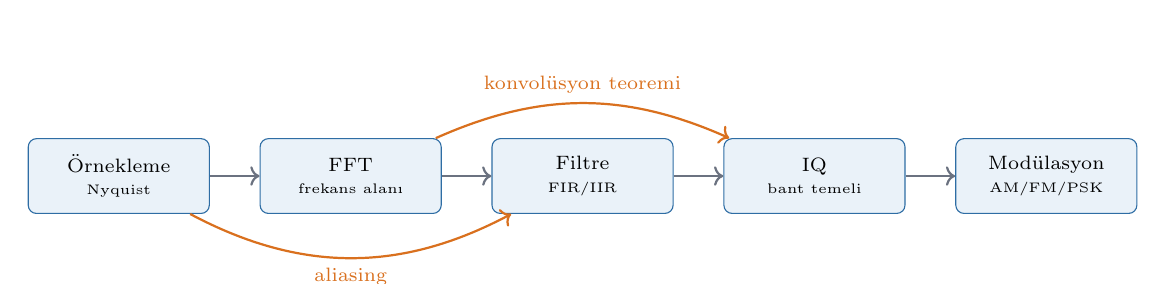
\begin{tikzpicture}[scale=0.95, every node/.style={font=\scriptsize},
  kutu/.style={draw=vurguMavi,fill=acikMavi,rounded corners=3pt,
               minimum width=2.3cm,minimum height=0.95cm,align=center}]
\node[kutu] (a) at (0,0) {Örnekleme\\ \tiny Nyquist};
\node[kutu] (b) at (3.1,0) {FFT\\ \tiny frekans alanı};
\node[kutu] (c) at (6.2,0) {Filtre\\ \tiny FIR/IIR};
\node[kutu] (d) at (9.3,0) {IQ\\ \tiny bant temeli};
\node[kutu] (e) at (12.4,0) {Modülasyon\\ \tiny AM/FM/PSK};
\foreach \x/\y in {a/b, b/c, c/d, d/e} \draw[->,thick,ortaGri] (\x)--(\y);
\draw[->,thick,turuncu] (a) to[bend right=28] node[below,turuncu]{aliasing} (c);
\draw[->,thick,turuncu] (b) to[bend left=24] node[above,turuncu]{konvolüsyon teoremi} (d);
\end{tikzpicture}
\end{center}

\begin{center}
\begin{tabularx}{\textwidth}{@{}>{\bfseries\color{anaMavi}}l >{\raggedright\arraybackslash}X >{\raggedright\arraybackslash}X@{}}
\toprule
\rowcolor{acikMavi}\multicolumn{1}{@{}l}{\color{anaMavi}\textbf{Kavram}} & \multicolumn{1}{l}{\color{anaMavi}\textbf{Sorduğu soru}} & \multicolumn{1}{l@{}}{\color{anaMavi}\textbf{Python karşılığı}}\\
\midrule
Örnekleme & Kaç hızda ölçmeliyim? & \code{np.arange}, \code{fs}\\
\rowcolor{acikGri} DFT/FFT & İçinde hangi frekanslar var? & \code{np.fft.rfft}\\
Filtre & Neyi geçireyim, neyi atayım? & \code{firwin}, \code{sosfilt}\\
\rowcolor{acikGri} IQ & Genlik ve faz ayrı ayrı ne yapıyor? & \code{hilbert}, \code{np.angle}\\
Desimasyon & Hızı nasıl düşürürüm? & \code{resample\_poly}\\
\rowcolor{acikGri} Modülasyon & Bilgiyi taşıyıcıya nasıl bindiririm? & \code{np.exp(1j*faz)}\\
Senkronizasyon & Faz ve saat nasıl kilitlenir? & PLL, Costas, Gardner\\
\bottomrule
\end{tabularx}
\end{center}

\ipucu{\textbf{Öğrenme yöntemi.} (1) Her kavramı önce \emph{üret}: bilinen bir
işaret sentezle. (2) Sonra \emph{ölç}: FFT'sini al, beklediğin yerde mi bak.
(3) Sonra \emph{boz}: gürültü, frekans ofseti, zamanlama hatası ekle ve
algoritmanın nerede çöktüğünü gör. (4) En son gerçek veriye geç. Bu sıra
izlendiğinde hata ayıklamak kolaydır; tersi sırada ise ``çalışmıyor'' der ve
nedenini asla bulamazsın.}

\vfill
\begin{center}
{\color{ortaGri}\rule{0.5\linewidth}{0.6pt}}\\[6pt]
{\color{ortaGri}\small Rehberin sonu --- İyi çalışmalar!}
\end{center}

\end{document}
